
%%%%%%%%%%%%%%%%%%%%%%%%%%%%%%%%%%%%%%%%%%%%%%%%%%%%%%%%%%%%%%%%%%%%%%%%%%%%%%%
%
%  EGSnrc manual: photon interactions
%  Copyright (C) 2015 National Research Council Canada
%
%  This file is part of EGSnrc.
%
%  EGSnrc is free software: you can redistribute it and/or modify it under
%  the terms of the GNU Affero General Public License as published by the
%  Free Software Foundation, either version 3 of the License, or (at your
%  option) any later version.
%
%  EGSnrc is distributed in the hope that it will be useful, but WITHOUT ANY
%  WARRANTY; without even the implied warranty of MERCHANTABILITY or FITNESS
%  FOR A PARTICULAR PURPOSE.  See the GNU Affero General Public License for
%  more details.
%
%  You should have received a copy of the GNU Affero General Public License
%  along with EGSnrc. If not, see <http://www.gnu.org/licenses/>.
%
%%%%%%%%%%%%%%%%%%%%%%%%%%%%%%%%%%%%%%%%%%%%%%%%%%%%%%%%%%%%%%%%%%%%%%%%%%%%%%%
%
%  Author:          Iwan Kawrakow, 2003
%
%  Contributors:    Blake Walters
%                   Frederic Tessier
%                   Ernesto Mainegra-Hing
%
%%%%%%%%%%%%%%%%%%%%%%%%%%%%%%%%%%%%%%%%%%%%%%%%%%%%%%%%%%%%%%%%%%%%%%%%%%%%%%%


\subsection{Photon interactions}
% Replace commented line for the one with fixed date when commiting
% Beware: Using the macro below conflicts between CVS and latex!!!
% \lfoot[{\sffamily {\leftmark}}]{{\small Last edited $Date: 2013/01/09 19:04:34 $
\lfoot[{\sffamily {\leftmark}}]{{\small Last edited 2011/05/02 18:36:27
}}

\subsubsection{Pair and triplet production}
\setcounter{equation}{0}
\label{pair}
\index{cross section!pair production}
\index{pair production}

\paragraph{Cross section} \hfill

The Feynman diagram for the production of electron-positron pairs 
in the nuclear field is given in Fig. \ref{pair_fig}. 
\begin{figure}[h]
%\begin{center}
%\setlength{\hsize}{15cm}
%\setlength{\vsize}{8cm}
%\setlength{\abovecaptionskip}{0.5in}
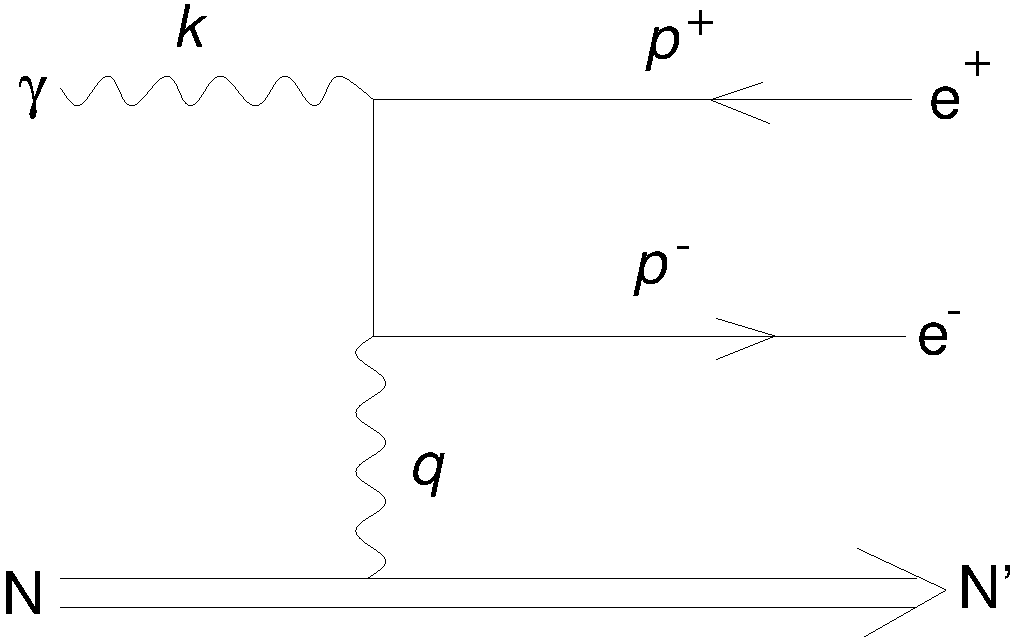
\includegraphics[height=8cm,width=12cm]{figures/pair}
\caption{\label{pair_fig} Feynman diagram for the pair 
production process}
%\end{center}
\end{figure}
The triplet production process is similar but the interaction 
takes place with one of the atomic electrons which receives 
sufficient energy to be set free (so that there are 3 secondary electrons 
produced in the interaction). By default 
the triplet production process is 
\index{triplet production}
not simulated explicitly but taken into account in an approximate 
way by using the total pair+triplet cross section to 
sample distances to subsequent pair production collisions.
By default EGSnrc adopts the cross sections used in EGS4, {\em i.e.} 
%total cross sections taken from ??? and 
extreme relativistic first Born approximation 
(Coulomb corrected above 50 MeV) 
differential cross sections  as formulated in the article by 
Motz, Olsen and Koch \cite{Mo69}. For a photon energy 
$k$ incident on the nucleus with the atomic number $Z$, the 
differential pair production cross section is
\begin{eqnarray}
\label{pair-e}
& & {{\rm d}\sigma_{\rm pair}(Z,k,E_+) \over {\rm d}E_+}  = 
{A_{\rm p}'(Z,k) r_0^2 \alpha Z (Z + \xi(Z) ) \over k} 
\\ & & \quad 
\left\{ \left( E_+^2 + E_-^2 \right) \left[ \phi_1(\delta) - 
{4 \over 3} \ln Z  - 4 \tilde{f}_c(k,Z) \right] + 
{2 \over 3} E_+ E_- \left[ \phi_2(\delta) - 
{4 \over 3} \ln Z  - 4 \tilde{f}_c(k,Z) \right] \right\} 
\nonumber
\end{eqnarray}
where $E_+$ and $E_-$ are the total energies of the 
positron and electron, 
\begin{equation}
\delta = 136 Z^{-1/3} 2 \Delta~,\quad \quad \Delta = {k m \over 2 E_+ E_-}
\end{equation}
and $\tilde{f}_c(Z)$ is the Coulomb correction,
\begin{equation}
\label{f_coulomb}
\tilde{f}_c(Z) =  
\begin{cases}
f_c(Z), & k \ge 50~\text{MeV} \\
0, & \text{else}
\end{cases}
\end{equation}
where $f_c(Z)$ was derived by 
Davies, Bethe and Maximon \cite{Da54},
\begin{equation}
\label{f_coulomb1}
f_c(Z) = a^2 \sum_{\nu=1}^\infty {1 \over \nu (\nu^2 + a^2)}, \quad 
a = \alpha Z~.
\end{equation} 
The empirical correction factor $A_{\rm p}'(k,Z)$ is 
introduced in order to improve the total pair production 
cross section at lower energies and is defined 
as ``The best estimate of the total cross section 
available divided by the total cross section resulting 
from the integration of Eq. (\ref{pair-e}) with 
$A_{\rm p}'(k,Z)=1$''. For energies above 
50 MeV $A_{\rm p}'$ is taken to be unity, for 
energies below 50 MeV the total pair+triplet cross sections compiled 
by Storm and Israel \cite{SI70} are used.
The replacement $Z^2 \to Z (Z + \xi(Z))$ takes 
into account the triplet production process, where $\xi(Z)$, 
evaluated by the PEGS4 function {\tt XSIF},  is given by 
\index{XSIF}
\begin{equation}
\xi(Z) = {L_{\rm rad}'(Z) \over L_{\rm rad}(Z) - f_c(Z)}
\end{equation}
where $f_c(Z)$ is defined in Eq. (\ref{f_coulomb}) and 
$L,L'$ are Tsai's radiation logarithms \cite{Ts74},
\index{Tsai's radiation logarithms}
\begin{eqnarray}
L_{\rm rad}'(Z) & = & 
\left\{
\begin{array}{r@{\quad , \quad}l}
\ln(1194\,Z^{-2/3}) &~~\mbox{if}~~~Z > 4 \\
6.144 & ~~\mbox{if}~~~Z = 1 \\
5.621 & ~~\mbox{if}~~~Z = 2 \\
5.805 & ~~\mbox{if}~~~Z = 3 \\
5.924 & ~~\mbox{if}~~~Z = 4
\end{array} \right. \nonumber \\
L_{\rm rad} & = & 
\left\{
\begin{array}{r@{\quad , \quad}l}
\ln(184.15\,Z^{-1/3}) &~~\mbox{if}~~~Z > 4 \\
5.310 & ~~\mbox{if}~~~Z = 1 \\
4.790 & ~~\mbox{if}~~~Z = 2 \\
4.740 & ~~\mbox{if}~~~Z = 3 \\
4.710 & ~~\mbox{if}~~~Z = 4 
\end{array} \right.
\end{eqnarray}
The functions $\phi_1(\delta)$ and $\phi_2(\delta)$, which 
account for screening effects, are 
given by 
\begin{equation}
\begin{split}
\phi_1(\delta) & = 4 \int\limits_\Delta^1 {{\rm d}q \over q^3} 
(q - \Delta)^2 \Big[1 - F(q,Z) \Big]^2 + 4 + {4 \over 3} \ln Z~,
\\ 
\phi_2(\delta) & = 4 \int\limits_\Delta^1  {{\rm d}q \over q^4} 
\Big[q^3 - 6 \Delta^2 q \ln \left({q \over \Delta}\right) + 3 \Delta^2 q 
-4 \Delta^3 \Big] \Big[1 - F(q,Z) \Big]^2 + {10 \over 3} + {4 \over 3} \ln Z
\end{split}
\end{equation}
where $q$ is the momentum transfer and $F(q,Z)$ the corresponding 
atomic form factor for an atom with atomic 
number $Z$. For a Thomas-Fermi potential $\phi_1(\delta)$ 
and $\phi_2(\delta)$ are independent of $Z$ and Butcher and 
Messel have approximated them \cite{BM60} as
\begin{eqnarray}
\label{pair_phi}
\phi_1(\delta) & = & \left\{
\begin{array}{r@{\quad , \quad}l}
20.867 - 3.242 \delta + 0.625 \delta^2 & \delta \le 1 \\
21.12 - 4.184 \ln(\delta + 0.952) & \delta > 1
\end{array}
\right. \\
\phi_2(\delta) & = & \left\{
\begin{array}{r@{\quad , \quad}l}
20.029 - 1.93 \delta - 0.086 \delta^2 & \delta \le 1 \\
\phi_1(\delta) & \delta > 1
\end{array}
\right.
\end{eqnarray}

The differential pair production cross section for compounds 
and mixture is derived from the independent atom approximation 
and can be approximately written in the same form as Eq. (\ref{pair-e}) 
but replacing 
\begin{eqnarray}
\label{pair_replace}
Z (Z + \xi(Z)) \quad & \mbox{with} & \quad Z_{\rm eff}^2 \equiv 
\sum p_i Z_i (Z_i + \xi(Z_i) ) 
\nonumber \\
{1 \over 3} \ln Z + \tilde{f}_c(k,Z) \quad & \mbox{with} & \quad 
Z_V \equiv \sum p_i 
Z_i (Z_i + \xi(Z_i) ) \left[ {1 \over 3} \ln Z_i + \tilde{f}_c(k,Z_i) \right] 
\nonumber \\
\delta \quad & \mbox{with} & \quad \delta_C 2 \Delta~,\quad 
\delta_C \equiv {136 \over Z_{\rm eff}^2} 
\sum p_i Z_i (Z_i + \xi(Z_i) ) Z_i^{-1/3} 
\end{eqnarray}
where $p_i$ is the normalized fraction of atoms of type $i$ in 
the molecule.

It is worth noticing that, due to the use of the extreme 
relativistic approximation,  the differential cross 
section as defined in Eq. (\ref{pair-e}) becomes inaccurate 
for energies close to the threshold energy for pair production 
(2 $\rm m$ ).  
%and breaks down altogether for energies below 
%2.1 MeV. 
In the EGS4 implementation, the entire photon energy 
was given to one of the pair particles for $k \le 2.1$ MeV. 
We have defined a macro {\tt \$SELECT-LOW-ENERGY-PAIR-PRODUCTION} 
which, in its default replacement, samples $E_+$ uniformly 
in the allowed range $m \cdots k/2$. If the user is aware 
of a better approach, this simplistic treatment can be 
modified by the appropriate replacement of this macro.   
\index{\$SELECT-LOW-ENERGY-PAIR-PRODUCTION}

\paragraph{NRC pair cross sections}\hfill
\index{pair cross sections!NRC}

In a more recent addition to EGSnrc, the user has the option
to specify use of a library of differential pair cross sections created
at the NRC. These cross sections are based on the exact partial-wave-analysis 
calculations by {\O}verb{\o}, Mork and Olsen (OMO) \cite{Ov73} for the 
unscreened nuclear potential modified by a multiplicative screening correction. 
The main difficulty in creating this data library, which provides cross 
sections up to 85 MeV for all elements between 1 and 100, consisted in finding 
numerically stable approaches for performing the PWA summation for energies 
above a few MeV (the OMO paper \cite{Ov73} only contains results up to 5.1 MeV). 
Note that these cross sections take into account the asymmetry in the
positron-electron energy distribution and eliminate the need
for the {\tt \$SELECT-LOW-ENERGY-PAIR-PRODUCTION} macro mentioned
above.

In order to make use of the NRC pair cross sections, the user
\index{pair\_nrc}
must set the variable {\tt pair\_nrc}=1.  Note that
{\tt pair\_nrc} is part of the {\tt COMIN/BREMPR} common block
(see Section~\ref{common_blocks} of this report).

\paragraph{Explicit simulation of triplet production}\hfill
\index{triplet production}

In a more recent addition to EGSnrc, the user has the option 
to explicitely simulate triplet production events according to the 
first Born approximation result first derived by Votruba \cite{Vo48} 
and later by Mork \cite{Mo67}. Due to the 3 particle final state the 
expression for the differential triplet production cross section 
is very complicated and so not reproduced here. It is worth 
noting that the published expressions most likely contain typos 
because their direct implementation in a computer program 
lead to meaningless results ({\em e.g.} negative cross section within 
the kinematically allowed range of energies and directions). 
The triplet production cross section was therefore re-derived using 
the CompHEP package, its results were manipulated using Mathematica and 
were then output directly to Fortran code. 

In order to turn on explicit simulation of triplet events, the user 
\index{itriplet} 
mist set the variable {\tt itriplet}=1. Note that
{\tt itriplet} is part of the {\tt COMIN/BREMPR} common block
(see Section~\ref{common_blocks} of this report).

The technique for sampling random directions and energies from 
the differential triplet cross section is very involved. 
Its detailed description awaits a future version of this report. 


\paragraph{Simulation of pair production, particle energies}\hfill
\index{pair production!simulation of}

When the NRC pair differential cross section tabulations are used, 
an alias table is employed for picking the positron energy. 
For the default Bethe-Heitler cross sections, 
the sampling algorithm implemented in EGS4 becomes extremely 
inefficient as the incident photon energy approaches the 
threshold energy. This is due to the following two facts: 
(i) The electron and positron energies, $E_-$ and $E_+$, 
are sampled in the range $0\cdots k/2$, the allowed 
range becomes a small fraction of the above interval for 
$k \to 2 m$. (ii) The rejection functions used are normalized 
to their maximum at $\delta = 0$. For photon energies that 
are not much larger than $2 m$ the actual possible maximum 
is much smaller.

\index{EGS4}
We have therefore slightly modified the EGS4 pair production sampling algorithm to improve 
its efficiency. If we define the functions 
\begin{eqnarray}
B(\delta) & = & 3 \Big[ \phi_1(\delta) - 4 Z_V \Big] - 
\Big[ \phi_2(\delta) - 4 Z_V \Big] \nonumber \\
C(\delta) & = & 3 \Big[ \phi_1(\delta) - 4 Z_V \Big] + 
\Big[ \phi_2(\delta) - 4 Z_V \Big] 
\end{eqnarray}
which will serve as rejection functions, and make 
a change of variables, 
\begin{equation}
\varepsilon  = {E_+ - m \over k - 2 m}~,
\end{equation}
the differential pair production cross section can be 
rewritten as 
\begin{equation}
{{\rm d} \sigma_{\rm pair} \over {\rm d} \varepsilon} = 
N \left\{ {B(\delta) \over B_{\rm max}} + \left(1 - {2 m \over k} \right)^2 
{A_{\rm max} \over 3 B_{\rm max}} A(\delta) 
\left[ 12 \left(\varepsilon - \frac{1}{2} \right)^2 \right] \right\}
\end{equation}
where $N$ combines all constant factors that are irrelevant for 
the sampling algorithm and $A_{\rm max}$ and $B_{\rm max}$ are 
the maxima of the rejection functions $A(\delta)$ and $B(\delta)$, 
\begin{equation}
A_{\rm max} = A\left({4 \delta_C m \over k}\right)~, \quad \quad 
B_{\rm max} = B\left({4 \delta_C m \over k}\right)~.
\end{equation}
The sampling algorithm, which determines the energy 
of the lower energy ``electron'' is then as follows:
\begin{enumerate}
\item
Calculate $A_{\rm max}$, $B_{\rm max}$ and $\alpha$,
\begin{equation}
\alpha = {1 \over 1 + (1 - 2 m/k)^2 A_{\rm max}/3/B_{\rm max}}
\end{equation}
To save time at high energies, use $A_{\rm max} = A(0)$ and 
$B_{\rm max} = B(0)$ for $k \ge 50$~MeV.
\item
Draw a random number $r_1$
\item
If $r_1 > \alpha$, then sample $\varepsilon$ 
from $12 (\varepsilon - 1/2 )^2$, {\em i.e.}
\begin{equation}
\varepsilon = \frac{1}{2} \left(1 - \mbox{Max}\{r_2,r_3,r_4\}\right)
\end{equation}
and use $A(\delta)/A_{\rm max}$ as a rejection function in step 5
\item
Else, sample $\varepsilon$ uniformly, {\em i.e.}
\begin{equation}
\varepsilon = \frac{1}{2} r_2
\end{equation}
and use $B(\delta)/B_{\rm max}$ as a rejection function in step 5
\item
Calculate $\delta$ and the rejection function $R$ = $A(\delta)/A_{\rm max}$ or 
$B(\delta)/B_{\rm max}$ 
\item
If $r_5 < R$, accept $\varepsilon$, else go to step 2.
\end{enumerate}

\begin{figure}[h]
%\setlength{\vsize}{12cm}
%\setlength{\abovecaptionskip}{0.5in}
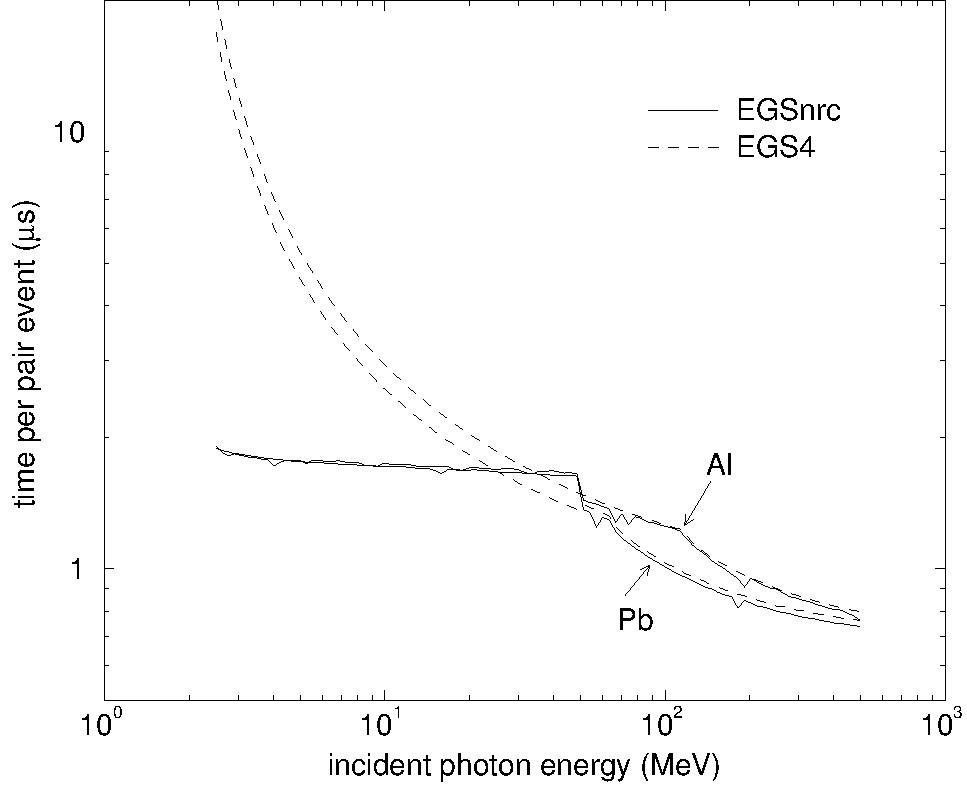
\includegraphics[height=12cm,width=12cm]{figures/pair_times}
\caption[CPU time for pair sampling]{\label{pair_times} 
CPU time in $\mu$s on a 500 MHz PIII computer to sample a pair energy.}
\end{figure}

Fig. \ref{pair_times} shows the CPU time in $\mu$s on a 500 MHz PIII computer 
running Linux necessary to sample a pair energy using the 
algorithms discussed here (solid lines) and the original EGS4 
algorithm (dashed lines) for aluminum and lead as a function 
of the incident photon energy (this is just the time for 
energy sampling, excluding angle sampling and rotations). Note 
the logarithmic scale and the dramatic increase in CPU time for 
the EGS4 algorithm and a photon energy less then 20 or 30 MeV. 
The discontinuity in the EGSnrc algorithm around $50$~MeV 
is due change in the 
approach to calculate $A_{\rm max}$ and $B_{\rm max}$  (see item 1).

\paragraph{Simulation of pair production, particle angles}\hfill
\index{pair production!angular distribution}

\index{Bielajew, Alex} \index{EGS4}
In the original EGS4 version electrons and positrons were 
produced at a fixed polar angle $\theta_{\pm}$ with respect to the direction 
of the incoming photon given by $\theta_{\pm}=m/k$. This approach 
was subsequently improved as discussed in PIRS Report 0287 
\cite{Bi91} which introduced the {\tt \$SET-PAIR-ANGLE} macro 
as an NRC extension to the EGS4 system. 
This macro is now included in the EGSnrc system. The angle 
selection procedure is controlled by the variable 
{\tt IPRDST} (part of the {\tt COMIN/EDGE} common block--
see Section~\ref{common_blocks}) which can assume the following values:
\index{IPRDST}
\begin{itemize}
\item[]{\tt IPRDST=0}: The original EGS4 approach is used, 
{\em i.e.} $\theta_{\pm}=m/k$
\item[]{\tt IPRDST=1}: The leading order term of the angular distribution 
is employed, {\em i.e.}
\begin{equation}
\label{pair_ang1}
{{\rm d} \sigma \over {\rm d} \Omega_\pm} = N 
{1 \over (1 - \beta_\pm \cos \theta_\pm)^2}
\end{equation}
where $N$ is again a normalization constant and $\beta_\pm$ denotes 
the velocity of the positron or electron in units of the speed of light.
\item[]{\tt IPRDST=2}: The formula 3D-2003 of the article by 
Motz {\em et al.} \cite{Mo69} is used, which is the cross section, differential 
\index{IPRDST}
in electron/positron energy and angle:
\end{itemize}
\begin{equation}
\label{pair_ang_2}
\begin{split}
{{\rm d} \sigma \over {\rm d} E_\pm {\rm d} \Omega_\pm} & =  
{N \over (u^2+1)^2 }
\left\{ -(E_+ - E_-)^2 - {16 u^2 E_+ E_- \over (u^2 + 1)^2} + 
\left[ E_+^2 + E_-^2 + {4 u^2 E_+ E_- \over (u^2 + 1)^2} \right] 
\ln M(k,E_\pm,u) \right\} \\
u & =  E_\pm \theta_\pm~, \quad {1 \over M(k,E_\pm,u)} = 
\left({k \over 2 E_+ E_-} \right)^2 + \left( { Z_{\rm eff}^{1/3} \over 
111 (u^2 + 1)^2 } \right)^2
\end{split}
\end{equation}
\begin{itemize}
\item[\phantom{\tt IPRDST=2}]
where all energies are measured in units of $m$. 
Note that Eq. (\ref{pair_ang_2}) is based on an extreme relativistic, 
small angle approximation where 
\begin{equation}
\begin{split}
(1 - \beta_\pm \cos \theta_\pm)^2 & \approx 
\left[1 - \beta_\pm \left(1 - \frac{\theta_\pm^2}{2}\right) \right]^2 
= (1 - \beta_\pm)^2 \left[ 1 - {\beta_\pm \over 1 - \beta_\pm} 
\frac{\theta_\pm^2}{2} \right]^2 \\
& \approx  (1 - \beta_\pm)^2 (1 + u^2)^2~.
\end{split}
\end{equation}
Perhaps, it would be a good idea to replace $1+u^2$ with 
$1 - \beta_\pm \cos \theta_\pm$ in the denominator outside 
of the curled brackets of Eq. (\ref{pair_ang_2}), but 
we have not undertaken this modification.   
\end{itemize} 

The sampling algorithm for Eq. (\ref{pair_ang_2}) is discussed 
extensively in Ref. \cite{Bi91}. 
\index{Bielajew, Alex}
%. 
It should be noted that 
this algorithm becomes progressively more inefficient with 
increasing energies. Given this fact and the approximations 
involved which make its use questionable at low energies, 
we have chosen {\tt IPRDST=1} as the default 
pair angle selection scheme in EGSnrc. The generation 
of electron and positron polar angles from the 
distribution (\ref{pair_ang1}) is trivial, it 
is accomplished by 
\index{IPRDST}
\begin{equation}
\cos \theta_\pm = {2 r - 1 + \beta_\pm \over \beta_\pm (2 r -1 ) + 1}
\end{equation}
where $r$ is an uniformly distributed random number between zero and 
unity. As pair-production is a three-body process, separate polar 
angles for the electron and positron are needed. The two 
azimuthal angles are chosen to be opposite. This is, 
strictly speaking, not correct, but due to lack of a better 
alternative, adopted from the original EGS4 version.

\paragraph{Russian Roulette for pair production events} \hfill
\index{Russian Roulette}
\index{variance reduction!Russian Roulette}
\index{pair production!Russian Roulette}

It is wasteful to simulate all pair production events if 
the user intends to play Russian Roulette with electrons 
set in motion in photon interactions. We have therefore implemented 
an EGSnrc internal Russian Roulette scheme which is turned on 
by setting the flag {\tt i\_play\_RR} which is in {\tt
COMIN/EGS-VARIANCE-REDUCTION/} 
to 1. The survival probability for the electrons is 
{\tt prob\_RR}, also in {\tt COMIN/EGS-VARIANCE-REDUCTION/}. 
If {\tt i\_play\_RR} is set, the following actions are 
taken at the beginning of subroutine {\tt PAIR}:
\index{EGS-VARIANCE-REDUCTION}
\index{prob\_RR} \index{i\_play\_RR}
\begin{enumerate}
\item
Pick a random number $r$
\item
If $r > $~{\tt prob\_RR}, reduce the stack size by one, return 
to {\tt PHOTON} ({\em i.e.} save the simulation of the pair event). 
If the stack becomes empty, a zero weight, zero energy photon 
is left on the stack so that the {\tt PHOTON} routine can exit 
properly.
\item
If $r < $~{\tt prob\_RR}, increase the weight of the current photon by 
1/prob\_RR and simulate the pair event as usual. 
\end{enumerate}
For more discussion of Russian Roulette see sections~\ref{rusrou} and
\ref{step_5b}.

\subsubsection{Incoherent (Compton) scattering}
\setcounter{equation}{0}
\label{compton}
\index{bound Compton scattering}
\index{Compton scattering}
\index{incoherent scattering}
\index{cross section!incoherent}

\paragraph{Cross section}\hfill

The Feynman diagram for the Compton scattering process is 
shown in Fig. \ref{compt_fig}. The circle in the line 
of the incoming atom A indicates that the electron 
\begin{figure}[h]
%\begin{center}
%\setlength{\hsize}{15cm}
%\setlength{\vsize}{8cm}
%\setlength{\abovecaptionskip}{0.5in}
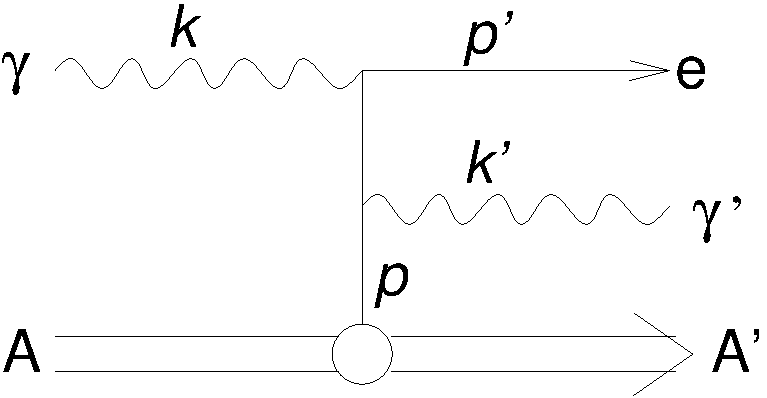
\includegraphics[height=8cm,width=12cm]{figures/compt}
\caption{\label{compt_fig} Feynman diagram for the Compton process}
%\end{center}
\end{figure}
is initially bound to the atom and represents the probability 
that an atomic electron with a four-momentum $p = (E,\vec{p})$ 
interacts with the incoming photon with a four-momentum 
$k=(k,\vec{k})$ into a final $e^-\gamma'$ state given by 
$k'=(k',\vec{k'})$ and $p'=(E',\vec{p}')$. 
To simplify the notation, all energies will be measured 
in units of the electron's rest energy $m$ and all momenta 
in units of $m/c$ in the following equations of this 
section. 

\index{Klein-Nishina}
If the binding to the atom is neglected and the electron 
is considered to be initially at rest ({\em i.e} $p = (1,0,0,0)$), 
the cross section for the process is given by the Klein-Nishina 
formula \cite{KN29},
\begin{equation}
{{\rm d} \sigma_{\rm KN} \over {\rm d} \cos \theta} = \pi r_0^2 Z~ 
X_{\rm KN}~, \quad \quad X_{\rm KN} = 
\left({k_c \over k} \right)^2 
\left[ {k_c \over k} + {k \over k_c} - \sin^2 \theta \right]
\end{equation}
where $\theta$ is the polar angle of the scattered photon with 
respect to the initial direction and $k_c$ is the energy 
of a photon scattered at an angle $\theta$ 
by free electrons at rest,
\begin{equation}
k_c = {k \over 1 + k (1 - \cos \theta)}
\end{equation}
\index{Doppler broadening}
\index{incoherent scattering!binding effects}
\index{incoherent scattering!Doppler broadening}
The treatment of the Compton process in EGS4 is based on these 
equations with $k' = k_c$. In EGSnrc we have included binding effects and 
Doppler broadening according to the impulse approximation (IA)
\cite{Ri75}. The IA assumes that the potential in which the 
target electrons move is constant so that their states can 
be represented by plane waves. The double differential 
cross section for photon scattering into the final state 
$k' = (k', k' \sin \theta \cos \phi, k' \sin \theta \sin \phi, \\
k' \cos \theta)$ is given by (Eq. (15) of Ref. \cite{RB82})
\begin{equation}
\label{comp_cs1}
{{\rm d}^2 \sigma_{\rm comp} \over {\rm d}k' {\rm d}\Omega} = 
{r_0^2 \over 2} {k' \over k q} \Big[1 + p_z^2 \Big]^{-1/2} X J(p_z)
\end{equation} 
where $\Omega$ is the solid angle $(\theta,\phi)$ and where
\begin{itemize}
\item
$q$ is the modulus of the momentum transfer vector 
$\vec{q} = \vec{k'} - \vec{k}$, 
\begin{equation}
q = \sqrt{k^2 + k^{\prime 2} - 2 k k' \cos \theta}
\end{equation}
\item
$p_z$ is the projection of the initial electron momentum 
on the direction of $\vec{q}$,
\begin{equation}
\label{comp_pz}
p_z = {\vec{p} \cdot \vec{q} \over q} = 
{k k' (1 - \cos \theta) - k + k' \over q}
\end{equation}
Note that the above equation is derived from a non-relativistic 
approximation and requires $|p_z| \le 1$.
\item
$X$ is defined as
\begin{eqnarray}
X & = & {R \over R'} + {R' \over R} + 
2 \left(\frac{1}{R} - \frac{1}{R'} \right) 
+ \left(\frac{1}{R} - \frac{1}{R'} \right)^2 \nonumber \\
R & = & k \left[ \sqrt{1 + p_z^2} + {k - k' \cos \theta \over q} p_z \right]
\nonumber \\
R' & = & R - k k' (1 - \cos \theta)~.
\end{eqnarray} 
Note that $R$ and $R'$ simplify to 
\begin{equation}
R \approx k \left(1 + O(p_z) \right)~, \quad 
R' \approx k \Big[1 - k_c (1 - \cos \theta ) \Big] \left(1 + O(p_z) \right) 
\end{equation}
for $p_z \ll 1$. In this limit 
\begin{equation}
X = X_{\rm KN} \left(1 + O(p_z) \right)
\end{equation}
\item
The function $J(p_z)$ is the Compton profile,
\begin{equation}
J(p_z) = \int {\rm d} p_x {\rm d} p_y | \psi(\vec{p}) |^2~,
\end{equation}
where $\psi(\vec{p})$ is the wave function of the bound electrons. 
Extensive tables of atomic and shell-wise 
\index{Compton profiles}
\index{incoherent scattering!Compton profiles}
Hartree-Fock Compton profiles for all 
elements have been published by Biggs {\em et al} \cite{BM75}.
Following Brusa {\em et al} \cite{BS96},  
contributions 
from different electron shells are considered separately, so 
that the atomic or molecular Compton profile is the sum 
of one-electron shell Compton profiles $J_i(p_z)$, and binding effects 
are taken into account by rejecting interactions that 
transfer less energy to the electron than the binding energy $U_i$,
{\em i.e.}
\begin{equation}
J(p_z) = \sum Z_i J_i(p_z) \Theta(k - k' - U_i)~.
\end{equation}
Here, $Z_i$ is the occupation number of shell $i$ and 
the $J_i$ have the normalization
\begin{equation}
\int\limits_{-\infty}^\infty {\rm d} p_z J_i(p_z) = 1
\end{equation} 
\end{itemize}
With all this, and after changing the cross section 
from differential in $k'$ to differential in $p_z$, 
Eq. (\ref{comp_cs1}) can be written as
\begin{equation}
{{\rm d}^2 \sigma_{\rm comp} \over {\rm d}p_z {\rm d}\Omega} = 
{r_0^2 \over 2} X_{\rm KN} 
\left( \sum Z_i J_i(p_z) \Theta(k - k' - U_i) \right) F(k,\cos \theta, p_z)
\end{equation}
where the function $F(k,\cos \theta, p_z)$ combines all remaining 
factors times ${\rm d}k'/{\rm d}p_z$,
\begin{equation}
F(k,\cos \theta, p_z) = \frac{k'}{k_c} \Big[ 1 + p_z^2 \Big]^{-1/2} 
\frac{X}{X_{\rm KN}} \left(1 + \frac{k_c}{k} {k \cos \theta - k' \over q} p_z 
\right)^{-1}
\end{equation} 
Here, $k'$ is a function of $k, \cos \theta$ and $p_z$ and 
follows from solving Eq. (\ref{comp_pz}) with respect to $k'$, 
{\em i.e.}
\begin{equation}
\label{comp_kprime}
k' = {k_c \over 1 - p_z^2 \varepsilon^2 } \left[ 
1 - p_z^2 \varepsilon \cos \theta + p_z \sqrt{1 - 2 \varepsilon 
\cos \theta + \varepsilon^2 \left(1 - p_z^2 \sin^2 \theta \right) }~ \right]~,
\quad \quad \varepsilon = \frac{k_c}{k}
\end{equation}
The incoherent scattering cross section, differential in 
the photon scattering angle, is 
\begin{equation}
\label{comp_sig_omega}
{{\rm d} \sigma_{\rm comp} \over {\rm d}\Omega} =
{r_0^2 \over 2} 
%\left(\frac{k_c}{k} \right)^2 : must not be there, noted by Trent Hawkins
X_{\rm KN} S(k,\cos \theta)
\end{equation}
where
\begin{equation}
\label{comp_sincoh}
S(k,\cos \theta) =  
\sum Z_i \Theta(k - U_i) S_i, \quad \quad 
S_i = \int\limits_{-\infty}^{p_i} {\rm d} p_z J_i(p_z) 
F(k,\cos \theta, p_z)
\end{equation}
\index{incoherent scattering function}
can be identified with the incoherent scattering function. 
The upper limit of the $p_z$ integration for the $i$'th shell, $p_i$,
\begin{equation}
\label{comp_pi}
p_i = { k (k - U_i) (1 - \cos \theta) - U_i \over 
\sqrt{ 2 k (k - U_i) (1 - \cos \theta) + U_i^2}}~,
\end{equation}
follows from Eq. (\ref{comp_pz}) with 
$k' = k - U_i$ and assures that sufficient energy is transferred 
to the electron to set it free. To first order, $S(k,\cos \theta)$ 
depends only on $k \sqrt{(1 - \cos \theta)/2}$ and so, 
Namito {\em et al} \cite{Na94} use tabulated 
incoherent scattering functions in their 
extension of the EGS4 system to include binding effects
and Doppler broadening, when sampling the photon scattering angle. 
This approach introduces a slight inconsistency in their treatment 
of the Compton process. 

As the Compton profiles are 
strongly peaked around $p_z=0$, the main contributions 
to the integral come from small $p_z$ values where 
the function $F(k,\cos \theta, p_z)$ is very close 
to unity and so, Brusa {\em et al} \cite{BS96} approximate 
$S(k,\cos \theta)$ with 
\begin{equation}
\label{comp_sincoh1}
S(k,\cos \theta) \approx S_A((k,\cos \theta) \equiv 
\sum Z_i \int\limits_{-\infty}^{p_i} {\rm d} p_z J_i(p_z)
\Theta(k - U_i)
\end{equation}
for their implementation of binding effects and Doppler broadening 
in the PENELOPE system \cite{Sa96}\footnote{They take 
into account $F(k,\cos \theta, p_z)$, using its Taylor 
expansion up to $O(p_z)$, for the sampling of $p_z$.}
\begin{figure}[h]
%\begin{center}
%\setlength{\vsize}{12cm}
%\setlength{\abovecaptionskip}{0.5in}
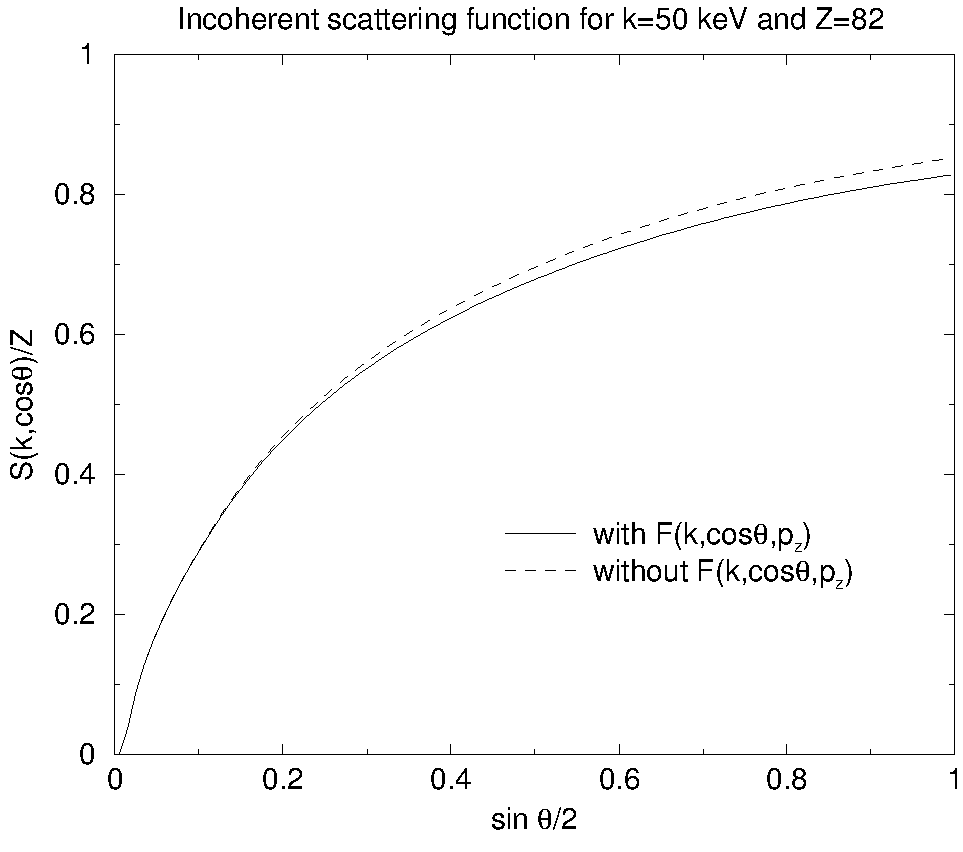
\includegraphics[height=12cm,width=12cm]{figures/sincoh}
%\end{center}
\caption[Incoherent scattering function]{\label{comp_sincoh_fig}
The incoherent scattering function for lead and $k=50$~keV 
calculated from Eq. (\protect\ref{comp_sincoh}) (solid line) 
and from Eq. (\protect\ref{comp_sincoh1}) (dashed line) 
by numerical integration}.
\end{figure}
This approach introduces a small error at low energies 
for high $Z$ materials as can be seen 
in Fig. \ref{comp_sincoh_fig} which shows 
$S(k,\cos \theta)$ for 50 keV photons in lead calculated 
with or without taking into account $F(k,\cos \theta, p_z)$.

To minimize the amount of data necessary for 
the simulation of the Compton process, and to make 
the calculation of the incoherent scattering function ``on the fly'' 
possible, we use 
the analytical approximations for the Compton profiles 
$J_i(p_z)$ proposed by Brusa {\em et al} \cite{BS96}:
\begin{equation}
\label{comp_Japprox}
J_i(p_z) = J_{i,0} (1 + 2 J_{i,0} |p_z| ) \exp\left[\frac{1}{2} - 
\frac{1}{2}\left(1 + 2 J_{i,0} |p_z| \right)^2\right]
\end{equation}
where $J_{i,0} \equiv J_i(0)$ is the value of the profile at 
$p_z = 0$ obtained from the Hartree-Fock orbital \cite{BM75}. 
In addition, we approximate $F(k,\cos \theta, p_z)$ by
\begin{equation}
\label{comp_Fapprox}
F((k,\cos \theta, p_z) = \left\{
\begin{array}{l@{\quad , \quad}l}
1 - \alpha p & p_z \le -p \\
1 + \alpha p_z & |p_z| < p \\
1 + \alpha p & p_z \ge p 
\end{array} \right.
\end{equation}
where 
\begin{eqnarray}
\label{comp_alpha}
\alpha & = & \frac{q_c}{k} \left(1 + 
{k_c (k_c - k \cos \theta) \over q_c^2} \right)
\nonumber \\
q_c & = & \sqrt{k^2 + k_c^2 - 2 k k_c \cos \theta}~.
\end{eqnarray}
Equation (\ref{comp_Fapprox}) results from a Taylor series 
expansion of $F(k,\cos \theta, p_z)$ up to $O(p_z)$. As this 
approximation becomes inaccurate for large $p_z$ values 
it is applied only for $|p_z| < p$, else the function values at 
$\pm p$ are used. We have checked by numerical integration 
of Eq. (\ref{comp_sincoh}) that the incoherent scattering function 
calculated with the approximation (\ref{comp_Fapprox}) agrees 
to better than 0.3\% with the incoherent scattering function 
calculated using the exact expression for $F(k,\cos \theta, p_z)$ 
if $p = 0.15$ is used. 

Combining now Eq. (\ref{comp_sincoh}), (\ref{comp_Japprox}) and 
(\ref{comp_Fapprox}),  we obtain for $S_i$
%\begin{equation}
%S_i(k,\cos \theta) = \left\{
%\begin{array}{l@{\quad , \quad}l}
%(1 - \alpha p) {e^{-b} \over 2} & p_z \le -p \\
%(1 + \alpha p_z) {e^{-b} \over 2} - {\alpha \over 4 J_{i,0}} 
%\sqrt{{\pi \over 2}} e^{1/2} \left[ \mbox{Erf} \left( 1 + 2 J_{i,0} p \over 
%\sqrt{2} \right) - \mbox{Erf} \left(  1 + 2 J_{i,0} |p_z| 
%\over \sqrt{2} \right) \right] & -p < p_z \le 0  \\
%1 - (1 + \alpha p_z) {e^{-b} \over 2} - {\alpha \over 4 J_{i,0}} 
%\sqrt{{\pi \over 2}} e^{1/2} \left[ \mbox{Erf} \left( 1 + 2 J_{i,0} p \over 
%\sqrt{2} \right) - \mbox{Erf} \left(  1 + 2 J_{i,0} |p_z| 
%\over \sqrt{2} \right) \right] & 0 < p_z < p \\
%1 - (1 + \alpha p) {e^{-b} \over 2} & p_z \ge p
%\end{array} \right.
%\end{equation}
\begin{eqnarray}
\label{comp_Si}
& & S_i(k,\cos \theta) \nonumber \\
& = & (1 - \alpha p) {e^{-b} \over 2}~,\quad \mbox{if}~~p_i \le -p \nonumber \\
& = &
(1 + \alpha p_i) {e^{-b} \over 2} - {\alpha \over 4 J_{i,0}} 
\sqrt{{\pi \over 2}} e^{1/2} \left[ \mbox{Erf} \left( 1 + 2 J_{i,0} p \over 
\sqrt{2} \right) - \mbox{Erf} \left(  1 + 2 J_{i,0} |p_i| 
\over \sqrt{2} \right) \right]~,\quad \mbox{else if}~~ p_i \le 0 \nonumber \\
& = & 
1 - (1 + \alpha p_i) {e^{-b} \over 2} - {\alpha \over 4 J_{i,0}} 
\sqrt{{\pi \over 2}} e^{1/2} \left[ \mbox{Erf} \left( 1 + 2 J_{i,0} p \over 
\sqrt{2} \right) - \mbox{Erf} \left(  1 + 2 J_{i,0} |p_i| 
\over \sqrt{2} \right) \right] ~,\quad \mbox{else if}~~ p_i < p \nonumber \\
& = &
1 - (1 + \alpha p) {e^{-b} \over 2} ~,\quad \mbox{else}
\end{eqnarray}
where
\begin{equation}
b = \frac{1}{2}\left(1 + 2 J_{i,0} |p_i| \right)^2 - \frac{1}{2}
\end{equation}
and $\mbox{Erf}$ is the error function. It is worth noticing that 
$S_i$ is always less or equal to unity. This fact allows for 
using it as a rejection function in the sampling algorithm discussed 
in the next section.

The total incoherent scattering cross section $\sigma_{\rm comp}^{\rm (tot)}$ 
can be obtained 
by a numerical integration over all scattering angles from 
Eq. (\ref{comp_sig_omega}), (\ref{comp_sincoh}) and 
(\ref{comp_Si}). To 
avoid substantial changes of the data preparation program PEGS4, 
we use instead the total Klein-Nishina cross section, 
$\sigma_{\rm KN}^{\rm (tot)}$, while tracking the photons through 
the geometry, and reject Compton interactions with the probability 
$1-\sigma_{\rm comp}^{\rm (tot)}/\sigma_{\rm KN}^{\rm (tot)}$ once 
at the interaction site (fictitious cross section method). 
This rejection probability results automatically (without 
calculating $\sigma_{\rm comp}^{\rm (tot)}$) from the sampling 
algorithm, as we shall see in the next section. 

\index{IBCMP}
Another advantage of this approach is that the user can 
turn on or off binding effects and Doppler broadening 
using the switch {\tt IBCMP} (included in the common
block {\tt COMIN/COMPTON-DATA}--see Section~\ref{common_blocks}), 
without preparing two 
separate material data files. The only additional data 
needed to simulate incoherent scattering in the impulse 
approximation are the Compton profile parameters 
$J_{i,0}$, taken from the tabulations by Biggs {\em et al} 
\cite{BM75}, and the occupation numbers $Z_i$ and 
binding energies $U_i$ for all elements, taken from 
Lederer and Shirley \cite{LS78}. These data are read in 
in subroutine {\tt init\_compton} which is called from 
{\tt HATCH}.
\index{init\_compton}

\paragraph{Simulation of incoherent scattering events}\hfill
\index{incoherent scattering!simulation of}
\index{Compton scattering!simulation of}
\index{bound Compton scattering}

The incoherent scattering cross section, differential in 
the photon scattering angle $\Omega = (\theta,\phi)$ 
and the Doppler broadening 
parameter $p_z$, per interaction site sampled from the 
total Klein-Nishina cross section is
\begin{eqnarray}
{{\rm d}^2 \sigma_{\rm comp} \over \sigma_{\rm KN}^{\rm (tot)}} & = &
\sum \frac{Z_i}{Z} \Theta(k - U_i)~ \sigma_i~ {\rm d} \Omega~ {\rm d} p_z 
\\ 
\sigma_i~ {\rm d} \Omega~ {\rm d} p_z & = & 
%\left( \int\limits_{-\infty}^{p_i} {\rm d} p_z J_i(p_z) F(k,\cos \theta,p_z)
%\right)~
S_i~
{{\rm d} \phi \over 2 \pi}~
{X_{\rm KN}(\cos \theta)~{\rm d} \cos \theta~ \over 
\int\limits_{-1}^1 X_{\rm KN}(\cos \theta) {\rm d} \cos \theta } 
~{ J_i(p_z) F(k,\cos \theta,p_z) \Theta(p_i - p_z) {\rm d} p_z \over 
\int\limits_{-\infty}^{p_i} {\rm d} p_z J_i(p_z) F(k,\cos \theta,p_z) }
\nonumber 
\end{eqnarray}
It is then clear that the following algorithm produces the 
required number of rejections and samples the differential 
cross section correctly, if the interaction is accepted:
\begin{enumerate}
\item
Sample the shell number $i$ using the probabilities $Z_i/Z$
\item
If the incident photon energy $k$ is smaller than the binding 
energy $U_i$, reject the interaction, 
else, sample $\cos \theta, \phi$ and $p_z$ using the differential 
cross section $\sigma_i$ of the selected shell as follows:
\item
Sample the photon polar scattering angle $\theta$ using 
\begin{displaymath}
P_1(\cos \theta) = 
{X_{\rm KN}(\cos \theta)~{\rm d} \cos \theta~ \over 
\int\limits_{-1}^1 X_{\rm KN}(\cos \theta) {\rm d} \cos \theta }
\end{displaymath}
which is a normalized probability distribution function (PDF). The method 
for sampling $\cos \theta$ will be explained below.
\item
Calculate the maximum possible value of $p_z$, $p_i$, from 
Eq. (\ref{comp_pi}), and $S_i$ from Eq. (\ref{comp_Si}).
\item
If a uniformly distributed random number is greater then $S_i$, 
reject the interaction
\item
Sample $p_z$ from 
\begin{displaymath}
P_2(p_z) = 
{ J_i(p_z) F(k,\cos \theta,p_z) \Theta(p_i - p_z) {\rm d} p_z \over 
\int\limits_{-\infty}^{p_i} {\rm d} p_z J_i(p_z) F(k,\cos \theta,p_z) }
\end{displaymath}
which is a normalized PDF for $p_z$. The sampling 
technique employed for this distribution function is explained below.
\item
Sample the azimuthal scattering angle from ${\rm d}\phi/(2 \pi)$
\item
Calculate the energy $k'$ of the scattered photon from 
Eq. (\ref{comp_kprime})
\item
The electron set in motion has then a kinetic energy of $k - k' - U_i$, 
a polar scattering angle $\theta_e$ given by 
\begin{equation}
\cos \theta_e = {k - k' \cos \theta \over 
\sqrt{k^2 + k^{\prime 2} - 2 k k' \cos \theta} }
\end{equation}
and an azimuth opposite to the photon's azimuth.
\end{enumerate}
Note that if the user does not want to take into account binding 
effects and Doppler broadening (the switch {\tt IBCMP} is set to zero)
the sampling algorithm consists of steps 3, 7 and 9 with 
$k' = k_c$ and $U_i = 0$. 
\index{IBCMP}

As the shell with which the interaction takes place is explicitly determined 
in step 1, at the end of the sampling algorithm the vacancy created 
by the Compton process is known. The relaxation of shell vacancies 
\index{relaxations}
\index{atomic relaxations}
with binding energies above the specified transport threshold 
energies is performed in subroutine {\tt relax} (see section \ref{relax}) and 
may lead to the creation of additional fluorescent photons and 
Auger and Coster-Kronig electrons on the stack. Many of the 
EGS4 based user codes assume that the outcome of an incoherent scattering 
process is a scattered photon and a Compton electron. This assumption 
is obviously not satisfied for EGSnrc, the outcome of an incoherent 
event may by any one of the following:
\begin{enumerate}
\item
The original photon, if the interaction was rejected due to the one 
of the rejection criteria
\item
A scattered photon and a Compton electron, if all relaxation particles 
had energies below the specified transport threshold energies 
({\tt ECUT} and {\tt PCUT})
\item
A scattered photon, a Compton electron plus $n$ relaxation particles, else.
\end{enumerate}
See section~\ref{stack_status} (page~\pageref{stack_status}) for more
information.

Finally, the portion of the binding energy that resulted in the creation 
of sub-threshold relaxation particles is made known to the user via 
a call to the scoring routine {\tt AUSGAB} with the argument {\tt IARG=4}. 
\index{AUSGAB}
\index{IARG!4}

We conclude this section with some details about steps 3, 4 and 6 
of the sampling algorithm.

\underline{Step 3, sampling of $\cos \theta$}: Following 
the EGS4 manual\cite{Ne85} we rewrite 
the PDF $P_1$ in terms of $\varepsilon = k_c/k$,
\index{SLAC-265}
\begin{equation}
\label{comp_P1}
P_1(\varepsilon) = P_1(\cos \theta) {{\rm d}\varepsilon \over 
{\rm d} \cos \theta} = N \left( \frac{1}{\varepsilon} + \varepsilon - 
\sin^2 \theta \right)
\end{equation}
where $N$ is a normalization constant that is irrelevant for the sampling 
algorithm. The minimum and maximum possible values for 
$\varepsilon$, $\varepsilon_{\rm min}$ and $\varepsilon_{\rm max}$, follow 
from $\cos \theta = -1$ and $\cos \theta = 1$, respectively, and are 
given by
\begin{equation}
\varepsilon_{{\rm min}} = {1 \over 1 + 2 k}~, \quad \quad 
\varepsilon_{{\rm max}} = 1~.
\end{equation}
Equation (\ref{comp_P1}) can be further rewritten as 
\begin{equation}
P_1(\varepsilon) = N (\alpha_1 + \alpha_2) \left\{
{\alpha_1 \over \alpha_1 + \alpha_2}~
\left({1 \over \varepsilon \alpha_1} \right)
+ {\alpha_2 \over \alpha_1 + \alpha_2}~\left({ \varepsilon \over \alpha_2}
\right) \right\} \left[ 1 - {\varepsilon \sin^2 \theta \over 1 + 
\varepsilon^2 } \right]
\end{equation}  
with 
\begin{equation}
\alpha_1  =  \ln \left(1 + 2 k \right)~, \quad \quad 
\alpha_2  = {1 - \varepsilon_{\rm min}^2 \over 2}
\end{equation}
$1/\varepsilon/\alpha_1$ and $\varepsilon/\alpha_2$ are 
normalized PDFs, they can be used to sample $\varepsilon$ 
with the probability $\alpha_1/(\alpha_1 + \alpha_2)$ and 
$\alpha_2/(\alpha_1 + \alpha_2)$, respectively. The expression 
of the square brackets has a maximum of unity for 
$\varepsilon = 1$ ($\sin \theta = 0$) and is thus 
a valid rejection function. The sampling algorithm is then as follows:
\begin{itemize}  
\item[3.1]
Calculate $\varepsilon_{\rm min}, \alpha_1, \alpha_2$ and 
$w = \alpha_1/(\alpha_1 + \alpha_2)$
\item[3.2]
Pick three random numbers $r_1, r_2$ and $r_3$ 
\item[3.3]
If $r_1 \le w$, 
\begin{equation}
\varepsilon = \varepsilon_{\rm min} \exp( r_2 \alpha_1 )~,
\end{equation}
else,
\begin{equation}
\varepsilon = \sqrt{ \varepsilon_{\rm min}^2 + 2 r_2 \alpha_2}
\end{equation}
\item[3.4]
Calculate the rejection function ($g$), if $r_3 > g$ go to step 3.2 
\item[3.5]
Deliver $\varepsilon$ (and $\cos \theta$)
\end{itemize}  
The efficiency of this algorithm 
goes to unity for $k \to \infty$ and therefore this is 
the most efficient algorithm at high incident photon energies.  
For $k \to 0$, the efficiency approaches $2/3$. In addition, 
the necessity to calculate a logarithm and an exponential function, 
two CPU intensive calculations, makes this algorithm slower than 
a simple rejection technique with a uniform sampling of $\varepsilon$. 
The rejection function in this case is given by
\begin{equation}
g = \frac{1}{g_{\rm max}} \left( {1 \over \varepsilon} + \varepsilon - 
\sin^2 \theta \right)~, \quad \quad g_{\rm max} = 
{1 \over \varepsilon_{\rm min}} + \varepsilon_{\rm min}
\end{equation}
and the algorithm is as follows
\begin{itemize}  
\item[3.1]
Calculate $\varepsilon_{\rm min}$ and $g_{\rm max}$
\item[3.2]
Pick two random numbers $r_1$ and $r_2$
\item[3.3]
Set 
\begin{equation}
\varepsilon = r_1 + (1 - r_1) \varepsilon_{\rm min}
\end{equation}
and calculate $g$
\item[3.4]
If $r_2 > g$, go to step 3.2
\item[3.5]
Deliver $\varepsilon$ (and $\cos \theta$)
\end{itemize}   
The efficiency of this algorithm is $2/3$ for low energies and 
decreases with increasing $k$. Because there are no CPU intensive 
calculations involved, it is faster up to $k \sim 2$ and 
used by EGSnrc in this energy range.

\underline{Step 4, calculation of $S_i$}: The calculation of 
$S_i$ requires two numerically intensive operations, the 
computation of $\exp(-b)$ and the calculation of the error 
function that depends on $p_i$. The former is necessary for 
the sampling of $p_z$ in step 6, the latter can be avoided 
by using an approximate formula for $\mbox{Erf}$ 
(Eq. 7.1.25 of Abramowitz and Stegun \cite{AS64}):
\begin{eqnarray}
& & e^{1/2} \mbox{Erf} \left( { 1 + 2 J_{i,0} |p_i| \over \sqrt{2} } \right) 
= e^{1/2} - e^{-b} t (a_1 + a_2 t + a_3 t^2 ) \\
t & = & {1 \over 1 + 0.332673 (1 + 2 J_{i,0} |p_i|)}~, \quad a_1 = 0.34802~, 
\quad a_2 = -0.0958798~, \quad a_3 = 0.7478556 \nonumber
\end{eqnarray}
which is accurate enough for our purposes.

\underline{Step 6, sampling $p_z$}: 
$p_z$ can be sampled using $J_i(p_z)$ as a PDF and $F$ as a rejection 
function. To determine the maximum of $F$ we note that $\alpha$ 
(given by Eq. (\ref{comp_alpha})) is always positive except for  
a small $\cos \theta$-range for $k > 3$. For such high incident 
photon energies the influence of $F$ is negligible and so 
we ignore it if $\alpha < 0$ ({\em i.e.} we set $\alpha = 0$).
The maximum of the rejection function, $F_{\rm max}$, is then
\begin{equation}
F_{\rm max} =   
\label{comp_Fmax}
 \left\{
\begin{array}{l@{\quad , \quad}l}
1 - \alpha p & p_z \le -p \\
1 + \alpha p_i & |p_i| < p \\
1 + \alpha p & p_i \ge p 
\end{array} \right.
\end{equation}
and the algorithm for sampling $p_z$ as follows:
\begin{itemize}  
\item[6.1]
Calculate $F_{\rm max}$ from Eq. (\ref{comp_Fmax})
\item[6.2]
Pick two random numbers, $r_1$ and $r_2$, calculate $r' = r_1 e^{-b}$ 
($e^{-b}$ is known from step 4 of the main algorithm)
\item[6.3]
Set 
\begin{equation}
p_z = \left\{ \begin{array}{l@{\quad , \quad}l} 
{1 - \sqrt{1 - 2 \ln [2 r']} \over 2 J_{i,0}} & r' < 1/2 \\
{\sqrt{1 - 2 \ln [2(1-r')]} - 1 \over 2 J_{i,0}} & r' \ge 1/2 
\end{array} \right.
\end{equation}
\item[6.4]
Calculate $F(p_z)$, if $r_2 > F(p_z)/F_{\rm max}$, go to step 6.2
\item[6.5]
Deliver $p_z$
\end{itemize}  
 
It is easy to see that the sampling of incoherent scattering events 
with binding effects and Doppler broadening taken into account 
requires substantially more numerical work compared to 
the free electron case (using the Klein-Nishina cross section). 
\begin{figure}[h]
%\setlength{\vsize}{12cm}
%\setlength{\abovecaptionskip}{0.5in}
%\epsfxsize = 12cm
%\epsfysize = 12cm
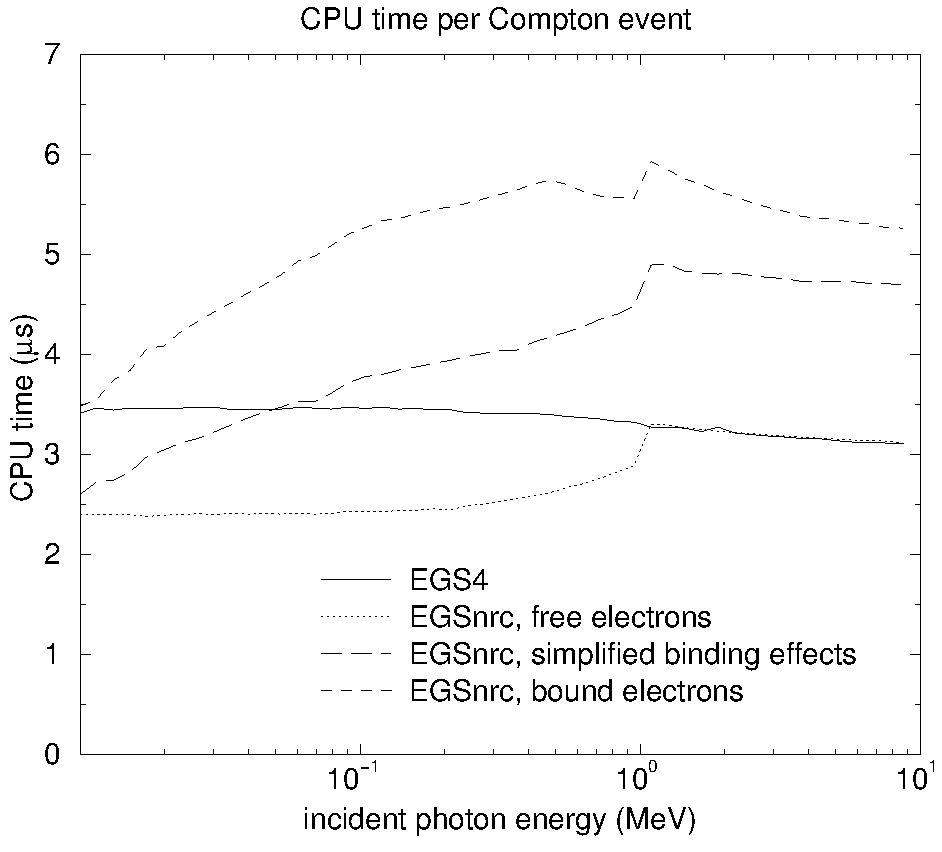
\includegraphics[height=12cm,width=12cm]{figures/comp_times}
\caption[CPU times for Compton sampling]{\label{comp_times}
CPU time in $\mu$s on a 500 MHz PIII computer to sample an incoherent 
scattering event (including necessary rotations of particle directions).}
\end{figure}
Fig. \ref{comp_times} shows the CPU time per incoherent scattering event 
for EGS4 (solid line), EGSnrc without (dotted line) 
and with binding effects (dashed line) as a function of the incident 
photon energy. The long dashed line would result if the function 
$F(k,\cos \theta,p_z)$ was ignored. EGSnrc without binding effects is 
faster than EGS4 for low photon energies due to the use of 
the uniform sampling technique. The inclusion of binding effects 
increases the CPU time per Compton event by not more than a 
factor of two and so has only a minor effect on the overall simulation 
time when electron transport is included. Binding effects and 
Doppler broadening for coherent scattering are therefore turned 
on by default in the {\tt block data} sub-program (the switch 
{\tt IBCMP} is set to unity).
\index{IBCMP}

Since the 2009 release of EGSnrc, the user has the option to change 
the EGSnrc behavior with respect to Compton interactions by 
setting {\tt ibcmp=2} or {\tt ibcmp=3}.
When {\tt ibcmp=2}, binding effects are taken into account via an 
incoherent scattering function, but there is no Doppler broadening.
This option was mainly added for the sake of being able to study the 
effect of Doppler broadening by comparing simulations with 
{\tt ibcmp=2} to {\tt ibcmp=1}. To select this option the user
must set {\tt Bound Compton scattering} to {\tt simple} in the
{\tt MC TRANSPORT PARAMETER} input block.
The {\tt ibcmp=3} option is the same as {\tt ibcmp=1}, but now the actual total 
bound Compton cross section 
is used and there are no rejections at run time. The addition of this option 
was motivated by the complications associated with the initial bound 
Compton scattering approach when using an un-weighting technique to compute 
ion chamber correction factors for photon attenuation. 
To select this option the user
must set {\tt Bound Compton scattering} to {\tt norej} in the
{\tt MC TRANSPORT PARAMETER} input block.

\index{Russian Roulette}
\index{variance reduction!Russian Roulette}
\index{incoherent scattering!Russian Roulette}
If the Russian Roulette option is turned on {\tt i\_play\_RR} set 
to 1, electrons produced as a result of the Compton interaction 
(the Compton electron and electrons from the relaxation of 
the shell vacancy) are removed from the stack with the probability 
{\tt prob\_RR}. If they survive, their weight is increased by 
1/{\tt prob\_RR}. 

\paragraph{Radiative Compton corrections}\hfill
\index{radiative Compton corrections}
\label{radc_corrections}

Recently, the code has been modified to also allow the user to include
radiative corrections for Compton scattering in the one-loop approximation. 
These corrections are based on the original 
Brown \& Feynman equations \cite{BF52}. The effect of loop corrections is to 
reduce the cross section at large photon scattering angles. This is partially 
offset by the addition of the double-Compton scattering process (two photons in 
the final state). Devising an efficient technique for sampling energies and 
directions from the double-Compton cross section is the most difficult part 
in the implementation. The method is quite involved and its detailed description 
awaits a future version of this report. 

In order to turn on radiative corrections, the input variable
\index{radc\_flag}
\texttt{radc\_flag} (in the common block \texttt{COMIN/COMPTON-DATA}) must be set to 1.
This option can be enabled in applications which can read the \texttt{MC transport parameter}
input block from an input file (\texttt{*.egsinp}) via the input key:
\begin{verbatim}
   Radiative Compton corrections = on
\end{verbatim}
Moreover, one must include the file \texttt{\$(EGS\_SOURCEDIR)rad\_compton1.mortran} to the
list of MORTRAN sources to be built just before \texttt{\$(EGS\_SOURCEDIR)get\_inputs.mortran}.
Depending on the application type this is accomplished in different ways:

\begin{itemize}
 \item
  For all C++ applications one must edit the file \texttt{\$HEN\_HOUSE/specs/egspp1.spec}
  and include the above file in the definition of the \texttt{C\_ADVANCED\_SOURCES}
  variable if the application is derived from the \texttt{EGS\_AdvancedApplication} class or the
  \texttt{C\_SIMPLE\_SOURCES} variable for any application derived from the \texttt{EGS\_SimpleApplication} class.
 \item
  For a specific C++ application one could define the variable \texttt{CPP\_SOURCES} in the application's
  \texttt{Makefile} in the same manner as done above for the \texttt{C\_ADVANCED\_SOURCES}.
 \item
  For a \texttt{BEAMnrc} application one must edit the file \texttt{sources.make} located in the application's
  folder and include the above file in the definition of the \texttt{SOURCES} variable
  or the \texttt{LIB\_SOURCES} variable if this \texttt{BEAMnrc} application will be used as a particle source for
  another application.
 \item
  For a MORTRAN application named for instance \texttt{app} one must edit the corresponding file app.make located
  in the application's folder \texttt{\$EGS\_HOME/app} and include the above file
  in the definition of the \texttt{SOURCES} variable.
\end{itemize}

% Note that if radiative Compton corrections are to be used then the \texttt{Makefile} of
% the user code must be modified to include the file \texttt{\$(EGS\_SOURCEDIR)rad\_compton1.mortran}
% in the \texttt{SOURCES} list, just before\\
% \texttt{\$(EGS\_SOURCEDIR)get\_inputs.mortran}.

\paragraph{Total Compton cross sections}\hfill
\label{comp_xsect}
\index{bound Compton scattering!user-supplied cross sections}

As mentioned above, the total Compton cross section used in EGSnrc is obtained 
from the theoretical expressions by integration of the differential cross sections. 
Another recent addition to the EGSnrc code allows the user to supply their
own cross sections for bound Compton scattering. This option is only available
if the user is simulating bound Compton scattering 
\index{IBCMP}
({\tt IBCMP}=1,2,3).  The cross sections
must be contained in a file\\
 {\tt \$HEN\_HOUSE/data/comp\_xsections\_compton.data},
where {\tt comp\_xsections} is the variable 
(in common block {\tt COMIN/MEDIA}) holding the name as supplied
by the user.
\index{comp\_xsections}

\subsubsection{Photo-electric absorption}
\setcounter{equation}{0}
\label{photo}
\index{photo-electric absorption}

In the photo-electric absorption process a photon is 
absorbed by an atom and an electron 
is emitted with an energy given by the incident photon 
energy minus its binding energy. 
The atom, left in an excited state with a vacancy in the 
ionized shell, relaxes via the emission of fluorescent photons and 
Auger and Coster-Kronig electrons.  

\index{fluorescent X-rays}
In the original default EGS4 implementation the emission of relaxation 
particles following photo-electric absorption events was 
ignored. This approach was later modified 
to include the production of $K_\alpha$ and $K_\beta$ fluorescent 
radiation. However, for incident photon energies below 
the $K$-shell binding energy, the entire photon energy is 
deposited locally. Another shortcoming of the EGS4 approach is 
that the $K$-shell binding energy is always subtracted 
from the energy of the electron set in motion, even though there 
is a certain probability that the photo-absorption process 
takes place with a shell other than the $K$-shell (for 
high-$Z$ materials this probability is of the order of 20\%). 
Finally, the use of the fluorescent option in EGS4 requires 
the user to select an ``effective'' atomic number for each 
material. The photo-absorption then always takes place with 
this atomic number. The meaningful selection of an 
``effective'' $Z$ proves to be a difficult task for mixtures, especially 
when only a small fraction of a high-$Z$ element is present.

\index{cross section!photo-electric absorption}
Although this release of EGSnrc uses the total photo-absorption 
cross sections from PEGS (which are taken from the 
compilation by Storm and Israel \cite{SI70}) 
the simulation of the photo-absorption process 
is completely changed and is controlled 
by the flag {\tt IEDGFL}
(in the {\tt COMIN/EDGE} common block-see Section~\ref{common_blocks}). If {\tt IEDGFL} of the 
region is non-zero, a detailed simulation is performed, 
otherwise a simplified treatment of the photo-absorption process 
is undertaken. The default setting of {\tt IEDGFL} is one. 
\index{IEDGFL}

\paragraph{Detailed simulation of photo-electric absorption}\hfill
\label{photo_detailed}
\index{photo-electric absorption!detailed simulation of}

\begin{enumerate}
\item
For compounds and mixtures, the first step is to sample the 
atomic number of the element the 
photon is interacting with.  
If $Z_i$ denotes the atomic number of the $i$'th element in 
the molecule, $p_i$ its stoichiometric index, and 
$\sigma_{\rm ph}(k,Z)$ the photo-electric absorption 
cross section for a photon of energy $k$ by an element 
with atomic number $Z$, then the probability $w_i(k)$ that 
the photon is absorbed by the element $Z_i$ is
\begin{equation}
w_i = {p_i \sigma_{\rm ph}(k,Z_i) \over \sum p_i \sigma_{\rm ph}(k,Z_i)}~.
\end{equation}
The sampling of the element therefore requires the knowledge of 
all elemental photo-absorption cross sections at run time, not 
just the total photo-absorption cross sections that comes from 
the PEGS data set. To minimize the amount of additional data 
required, we use fit formulas for the $\sigma_{\rm ph}(k,Z_i)$'s 
which are accurate to within 1-2\% and have the form
\begin{eqnarray}
\sigma_{\rm ph}(k,Z) & = & \frac{A_K(Z)}{k} + \frac{B_K(Z)}{k^2} + 
\frac{C_K(Z)}{k^{7/2}} + \frac{D_K(Z)}{k^4}~, \quad \mbox{if}~k \ge U_K(Z)
\\
%& = & \exp \left[A_j(Z) + B_j(Z) \ln k + C_j(Z) (\ln k)^2 + D_j(Z) (\ln k)^3 
%\right]~, \quad \mbox{else if}~k \ge U_j(Z)
& = & \exp \left[A_j(Z) + B_j(Z) t + C_j(Z) t^2 + D_j(Z) t^3 
\right]~, \quad \mbox{else if}~k \ge U_j(Z)
\nonumber 
\end{eqnarray}
where $t = \ln k$ and where $U_K(Z)$ is the 
$K$-shell binding energy and $U_j(Z)$ binding 
energies for shells other then the $K$-shell. We have obtained The 
coefficients $A_K, B_K, ...$ and $A_j, B_j, ...$  
by fitting the photo-absorption cross sections from the {\tt XCOM} program 
\cite{BH87} and are found in the file {\tt photo\_cs.data} 
(only shells with a binding energy above 1 keV are included). 
The algorithm to select the element that absorbs the 
incident photon is then:
\begin{itemize}
\item[1.1] Calculate all $\sigma_{\rm ph}(k,Z_i)$ and 
their sum
\item[1.2] Pick a random number $r_1$
\item[1.3] In a loop over the number of elements, calculate 
$r_1 = r_1 - w_i$, if $r_1 \le 0$ exit the loop and take 
$Z_i$ as the element interacting with the photon. 
\end{itemize}
Note that, at least in principle, 
\begin{displaymath}
\sum p_i \sigma_{\rm ph}(k,Z_i) = \sigma_{\rm ph}(k)
\end{displaymath}
where $\sigma_{\rm ph}(k)$ is the photo-absorption cross section 
for the material under consideration. This cross section is 
interpolated using the PEGS supplied data in the photon 
transport routine in order to determine 
the interaction type. One could make the element selection algorithm 
more efficient by employing 
\begin{itemize}
\item[1.1']
Pick a random number $r_1$
\item[1.2']
Set $i=1$
\item[1.3']
Calculate $\sigma_{\rm ph}(k,Z_i)$ and 
$r_1 = r_1 - p_i \sigma_{\rm ph}(k,Z_i)/\sigma_{\rm ph}(k)$.
\item[1.4'] If $r_1 > 0$ and $i$ less then the number of elements, 
then $i = i+1$, go to step 1.3'.
\item[1.5'] Deliver $i$.
\end{itemize}
as this saves the evaluation of one or more $\sigma_{\rm ph}(k,Z_i)$ 
(especially if elements are ordered by decreasing probability for 
photo-absorption prior to the actual simulation). We have not 
implemented this more efficient algorithm as the photo-absorption 
cross section interpolated using the PEGS supplied data becomes 
inaccurate around absorption edges. This potential improvement is 
left for future releases of the system (which are anticipated to 
not make use of PEGS data sets).
\item
Once the absorbing element is determined, the shell 
with which the interaction takes place has to be sampled. 
The probability $\nu_j$ that the photon is absorbed by the $j$'th shell 
is close to energy independent for the $K$-shell but depends  
on the incident photon energy for other shells. This means that 
shell-wise photo-absorption cross sections would be required 
to be available at run time in order to sample the shell 
if one wanted to perform a complete modeling of the 
photo-absorption process. In this release of the EGSnrc system 
we use instead energy independent interaction probabilities $\nu_j$ 
which are determined as follows. If $\phi(k)$ is the 
fluence of the photon radiation field, the number of photo-absorption 
events by the element $Z$ per unit volume, $N$, is given by
\begin{equation}
N = n(Z) \int {\rm d} k \phi(k) \sigma_{\rm ph}(k,Z)
\end{equation}
where $n$ is the density of scattering centers. 
The number of photo-absorptions by the shell $j$ of this 
element per unit volume is
\begin{equation}
N_j = n(Z) \int {\rm d} k \phi(k) \sigma_{{\rm ph},j}(k,Z)
\end{equation}
where $\sigma_{{\rm ph},j}(k,Z)$ is the photo-absorption cross section 
of the $j$'th shell. The ratio of $N_j$ to $N$ is the average 
interaction probability for absorption by the $j$'th shell, $\nu_j'$, 
for the radiation field described by $\phi(k)$,
\begin{equation}
\nu_j' = \frac{N_j}{N} = {\int {\rm d} k \phi(k) \sigma_{{\rm ph},j}(k,Z) 
\over \int {\rm d} k \phi(k) \sigma_{\rm ph}(k,Z) }
\end{equation}
The actual quantity used in the simulation of photo-electric absorption 
is the probability $\nu_j$ that the photon is absorbed by the 
shell $j$  if it was not absorbed by one of the shells $1 \cdots j-1$,  
which is given by
\begin{equation}
\label{photo_nuj}
\nu_j = {\int {\rm d} k \phi(k) \sigma_{{\rm ph},j}(k,Z) \over 
\sum_{i=j}^{N_{\rm sh}} \int {\rm d} k \phi(k) \sigma_{{\rm ph},i}(k,Z)}
\end{equation}
where $N_{\rm sh}$ is the total number of shells. 
To calculate $\nu_j$ one needs $\phi(k)$, a quantity that 
is not known (but intended to be calculated by the Monte 
Carlo simulation). Nevertheless, one could calculate 
$\nu_j$ by making a guess about the photon fluence, this 
approach is the basis for the generation of group interaction 
coefficients for discrete ordinate methods (see {\em e.g} 
the book by Lewis and Miller \cite{LM84}). 
\begin{figure}[h]
%\setlength{\vsize}{12cm}
%\setlength{\abovecaptionskip}{0.5in}
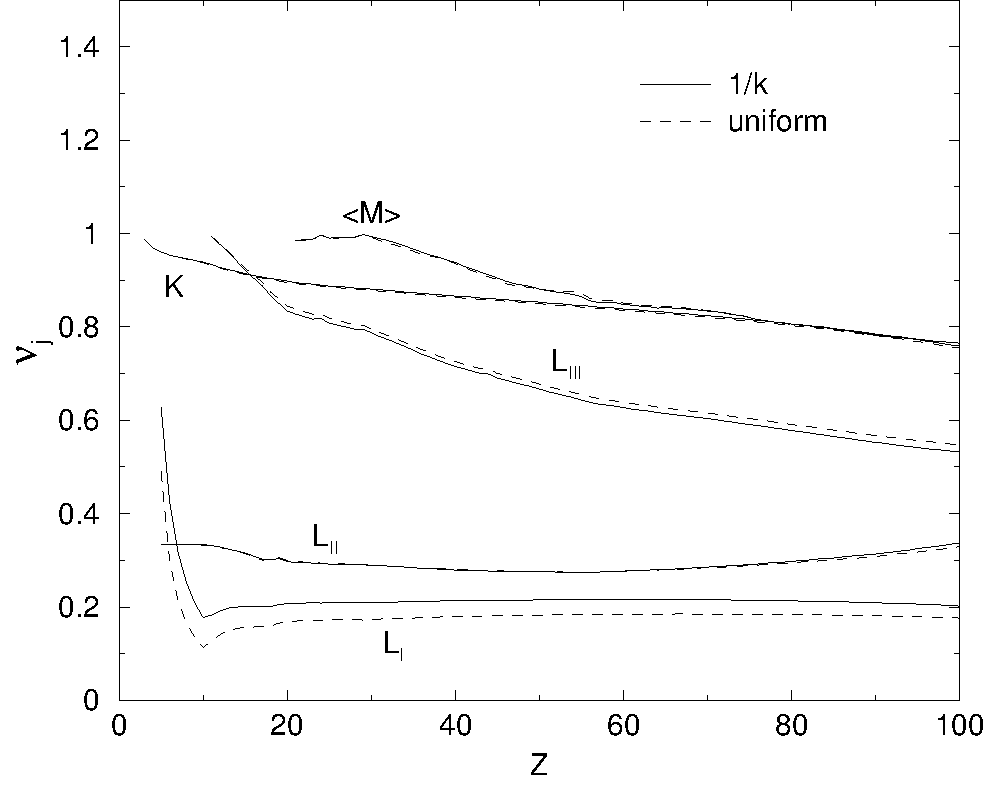
\includegraphics[height=12cm,width=12cm]{figures/intp}
\caption[Interaction probabilities for different shells]{\label{phot_intp}
Interaction probabilities $\nu_j$ for different shells as 
calculated from Eq. (\protect\ref{photo_nuj}) using 
$\phi(k)=1/k$ (solid lines) or $\phi(k)=\mbox{const}$ (dashed lines).}
\end{figure}
Figure \ref{phot_intp} shows the interaction probabilities 
$\nu_j$ of the $K, L_I, L_{II}$ and  $L_{III}$ shells and an 
``average'' $M$ shell (see next paragraph) 
as a function of the 
atomic number $Z$ for $\phi(k) = \mbox{const}$ (dashed line) 
and $\phi(k) = \mbox{const}/k$ (solid line). 
Shell-wise photo-absorption cross section from 
the Evaluated Photon Data Library (EPDL) \cite{Cu89} 
were used to generate this figure, the upper limit of 
the $k$-integration was set to 1 MeV. The dependence of 
the $\nu_j$s on the weighting function $\phi(k)$ is 
negligible except for the $L_I$ shell where the difference 
is of the order of 10\%. This fact was the motivation for 
using the energy independent interaction probabilities $\nu_j$, 
a better approach is scheduled for a future release of the 
system. 
 
The use of an interaction probability for an ``average'' $M$-shell 
is motivated by the fact that relaxation transitions from and to 
$M$-shells are treated in an average way, see section \ref{relax}.
Given the definition of the $\nu_j$'s, $\nu_{\langle M \rangle}$ is 
\begin{equation}
\nu_{\langle M \rangle} = 1 - \prod (1 - \nu_{M_i})
\end{equation}
where the product runs over the number of $M$-sub-shells available 
for the element $Z$ (up to 5). The interaction probabilities 
$\nu_K, \nu_{L_I}, \nu_{L_{II}}, \nu_{L_{III}}$ and $\nu_{\langle M \rangle}$, 
calculated with the $1/k$ weighting function, are stored in the 
file {\tt photo\_relax.data} and read in by the subroutine 
{\tt edgset} which is called from {\tt HATCH}.

With all this, the algorithm for selecting the shell that absorbs 
the incident photon is as follows:
\begin{itemize}
\item[2.1]
Determine the inner-most shell $j$ that has a binding energy lower 
than the incident photon energy and pick a random number $r_2$
\item[2.2]
If $r_2 < \nu_j$ or $j > \langle M \rangle$
\footnote{The outer-most shell treated is the $M$ shell, if the photon
was not absorbed by it, it is assumed that it is absorbed by the
$N$ shell.}, then deliver $j$
\item[2.3]
Set $r_2 = (1 - r_2)/(1 - \nu_j),~j = j+1$, go to step 2.2
\end{itemize} 
\item
Once the element and its shell absorbing the photon is determined, 
a photo-electron with the kinetic energy $k - U_j(Z)$ is set-up, where 
$U_j(Z)$ is the binding energy of the selected shell. 
The vacancy created is treated in the routine ({\tt relax}, see section 
\ref{relax}), 
this significant change compared to EGS4 is motivated by the 
fact that shell vacancies are created also
in other processes, {\em e.g.} Compton scattering (see section \ref{compton}).
The sampling of the photo-electron direction is discussed in section 
\ref{photo_direction}.
\end{enumerate}

\paragraph{Simplified simulation of photo-electric absorption}\hfill
\label{photo_simple}
\index{photo-electric absorption!simplified simulation of}

If the flag {\tt IEDGFL} for the current region is set to zero, 
a simplified simulation of the photo-absorption process is undertaken. 
This simplified treatment consists of one step:
\index{IEDGFL}
\begin{enumerate}
\item
Set-up a photo-electron with a kinetic energy $k$
\end{enumerate}
There are several reasons which motivated us to change the 
logic compared to the current EGS4 version (where the 
$K$-shell binding energy is always subtracted):
\begin{itemize}
\item
The treatment is greatly simplified
\item
If the flag {\tt IEDGFL} is set to zero, it is reasonable to assume 
that the detailed calculation of the spread of energy released 
in photo-absorption events is not important for the situation 
under investigation
\item
The effect of the production of relaxation particles in the 
de-excitation cascade following photo-electric absorption is 
to spread out the binding energy around the point of interaction. 
By giving the photo-electron the entire incident photon energy, 
this effect is at least partially simulated.
\end{itemize}
 
\paragraph{Photo-electron direction}\hfill
\label{photo_direction}
\index{photo-electric absorption!direction of electron}

\index{IPHTER}
The behavior of the sampling of the photo-electron direction 
is controlled by the switch {\tt IPHTER} 
(included in the {\tt COMIN/EDGE} common block) which set on a 
region by region basis. If set to zero, 
the photo-electron ``inherits'' the direction of the incident 
photon. If set to non-zero (the default selection), 
the direction is sampled from the 
Sauter distribution \cite{Sa31}. The implementation as discussed 
in detail in Ref. \cite{BR86a} is adopted. For completeness, we give a 
brief summary here.
\index{Bielajew, Alex}

Sauter's distribution in the polar angle 
$\mu = \cos \theta$ with respect to the incident 
photon direction may be cast in the form \cite{BR86a}
\begin{equation}
f(\mu) {\rm d}\mu = {1 - \mu^2 \over (1 - \beta \mu)^4} \left[ 1 + 
\kappa (1 - \beta \mu) \right] {\rm d} \mu
\end{equation}
where $\beta$ is the electron's velocity in units of the 
speed of light  and 
\begin{equation}
\kappa = {\gamma \over 2} (\gamma - 1) (\gamma - 2)~, \quad \gamma = 
{1 \over \sqrt{1 - \beta^2} }
\end{equation}
This equation can be sampled by generating candidate 
$\mu$ values from 
\begin{equation}
g(\mu) = {1 \over 2 \gamma^2 (\kappa + \gamma)^2} ~{
1 + \kappa (1 - \beta \mu) \over (1 - \beta \mu)^2 }~,
\end{equation}
which is a normalized PDF for $\mu$, and using 
\begin{equation}
h(\mu) = { \gamma + 1 \over 2 \gamma } ~{1 - \mu^2 \over 1 - \beta \mu }
\end{equation}
which is always positive and has a maximum of unity, 
as a rejection function. To generate $\mu$ values from 
$g(\mu)$, one uses
\begin{equation}
\mu = {1 \over \beta} \left[1 - \left( \sqrt{\left(\kappa + {1 \over 1 + \beta}
\right)^2 + 4 \beta \gamma^2 (\kappa + \gamma^2) r_1} - \kappa \right)^{-1} 
\right]
\end{equation}
where $r_1$ is an uniformly distributed random number. 

\index{Sauter distribution}
It is worth noticing that, strictly speaking, Sauter's distribution is 
valid only for the $K$-shell and also derived 
from an extreme relativistic approximation. The treatment 
of the photo-electron angular distribution is therefore left 
as a macro {\tt \$SELECT-PHOTOELECTRON-DIRECTION;} 
and can therefore be replaced, if the user has a better approach.
\index{\$SELECT-PHOTOELECTRON-DIRECTION}

\subsubsection{Coherent (Rayleigh) scattering}
\label{rayleigh}
\setcounter{equation}{0}
\index{Rayleigh scattering}
\index{coherent scattering}
\index{cross section!coherent}

Originally, EGSnrc ``inherited'' the treatment of the coherent 
photon scattering process from EGS4 \cite{Ne85}. 
This means that the total coherent scattering cross 
sections from Storm and Israel \cite{SI70} and the atomic 
form factors $F_T(q,Z)$ from Hubbel and {\O}verb{\o} \cite{HO79} are used 
by default. 
The form factors for molecules are calculated from the independent 
atom approximation, {\em i.e.}
\begin{equation}
[F_T(q)]^2 = \sum p_i [F_T(q,Z_i)]^2
\end{equation}
where $p_i$ is the stoichiometric index of the $i$'th element,  
$Z_i$ its atomic number and $q$ the momentum transfer when 
a photon with an energy $k$ is scattered by an angle $\theta$, 
\begin{equation}
q = k \sqrt{{1 - \cos \theta \over 2}}~.
\end{equation}
The coherent scattering cross section, differential in the 
photon angle $\Omega = (\theta, \phi)$ is
\begin{equation}
{{\rm d} \sigma_{\rm R} \over {\rm d} \Omega} = {r_0^2 \over 2} 
(1 + \cos^2 \theta) [F_T(q)]^2~.
\end{equation}
This equation is sampled by re-writing it in terms of 
$q^2$,
\begin{equation}
{{\rm d} \sigma_{\rm R} \over {\rm d} q^2} = {4 \pi r_0^2 \over k^2}~
A(q_{\rm max}^2)~
{1 + \cos^2 \theta \over 2} ~{[F_T(q)]^2 \over A(q_{\rm max}^2)
}
\end{equation}
where 
\begin{equation}
A(q^2) = \int\limits_0^{q^2} {\rm d}q^{'2} [F_T(q')]^2
\end{equation}
and $q_{\rm max} = k$ is the maximum possible momentum transfer, and 
using $[F_T(q)]^2/A(q_{\rm max}^2)$  as a PDF for $q^2$ and 
$(1 + \cos^2 \theta)/2$ as a rejection function.

\index{coherent scattering!sampling of}
\index{IRAYLR}  \index{\$RAYLEIGH-SCATTERING;}
The actual sampling, accomplished in the macro 
{\tt \$RAYLEIGH-SCATTERING;}, is performed only 
if the switch {\tt IRAYLR} (included
in the {\tt COMIN/MISC} common block--see Section~\ref{common_blocks}) 
is set to non-zero for the current 
region. By default, {\tt IRAYLR} is set to zero in the {\tt 
block data} subprogram. The motivation for this choice is 
the fact that the {\tt \$RAYLEIGH-SCATTERING;} macro 
requires the function $A(q^2)$ to be included in the PEGS data
set. This additional data is only included, if the user specifically
requested it from PEGS. 

We recommend the Rayleigh 
scattering option to be used for low energy calculations 
(say, below 1 MeV). It is worth noticing that 
inclusion of coherent scattering without the use 
of the bound Compton scattering option (see section \ref{compton}) 
results in too much photon scattering, binding effects 
for incoherent scattering should therefore always be turned 
on if the Rayleigh option is used.

\paragraph{New coherent scattering angular sampling}\hfill
\label{new_rayleigh_sampling}

\index{Rayleigh scattering!new angular sampling}
% The above sampling algorithm approximates the angular distribution 
% for coherent scatter relatively well. However,
% the forward peaked shape of $[F_T(q)]^2/A(q_{\rm max}^2)$
% and its uniform sampling in equidistant intervals 
% between 0 and 1 translates into a non-uniform sampling
% of the scattering angle since larger angular intervals
% are covered with increasing bin number. As a consequence,
The original EGS4 sampling algorithm produces a step-like averaging 
artifact at large angles, which increases with energy. This is 
shown by the symbols in Figure \ref{ray_ang_sampling_fig}, for 
20 keV, 60 keV and 110 keV photon beams in water. 
However, this artifact has no practical consequences, unless one is 
interested in the few photons scattered at large angles.
\begin{figure}[h]
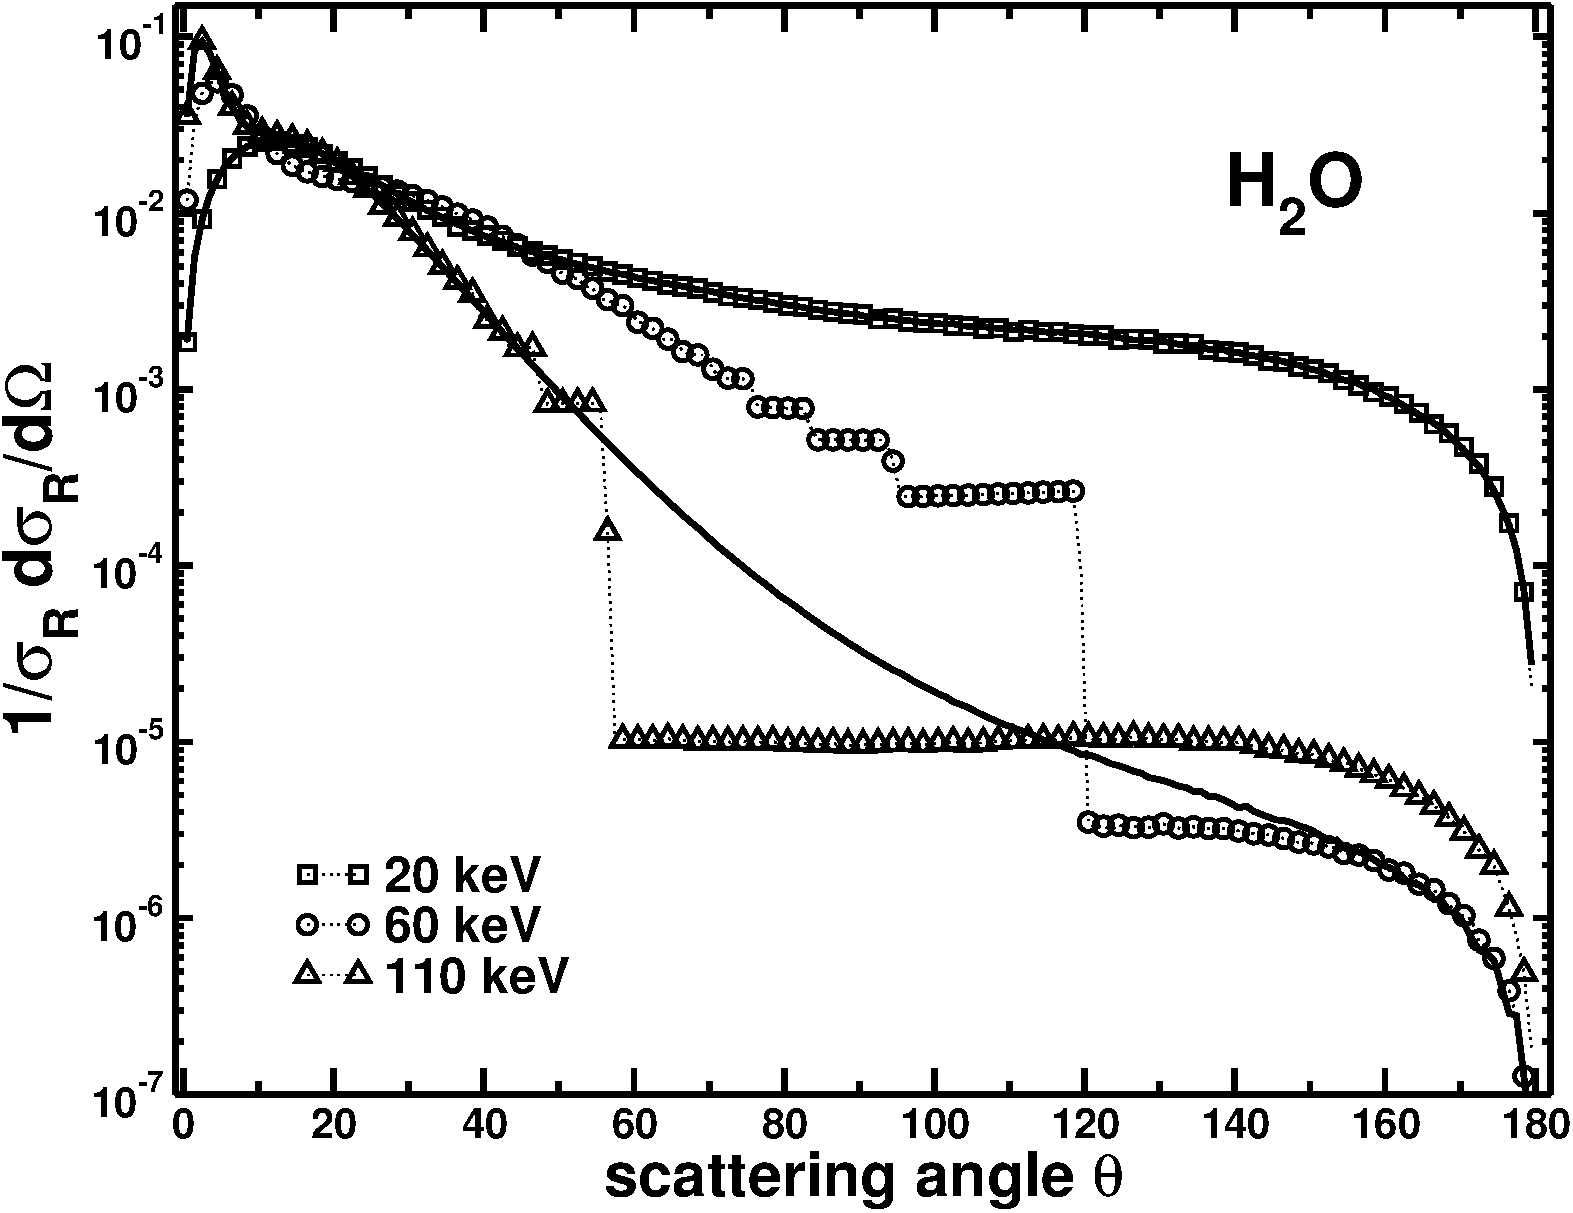
\includegraphics[height=9cm,width=9cm]{figures/ray_ang_dist_old_vs_new}
\caption[Angular distribution of coherently scattered photons for 20 keV, 60 keV 
and 110 keV photon beams in water.]{\label{ray_ang_sampling_fig}
Angular distribution of coherently scattered photons for 20 keV, 60 keV 
and 110 keV photon beams in water. Symbols represent the original EGS4
sampling algorithm and the solid lines the new alias sampling.
}
\end{figure}

The default angular sampling algorithm for coherent scattering 
was replaced in 2007 for an alias-sampling algorithm that properly 
samples $[F_T(q)]^2/A(q_{\rm max}^2)$ removing this artifact as shown
by the solid lines in Figure \ref{ray_ang_sampling_fig} for 20 keV
and 110 keV. The coherent scattering form factors are now
read directly either from {\tt \$HEN\_HOUSE/pegs4/pgs4form.dat} 
(default atomic form factors, see section \ref{rayleigh} above) or from
user-supplied form factor files expected to be in the
{\tt \$HEN\_HOUSE/data/molecular\_form\_factors/} directory
(see section \ref{custom_ff_sect} below for more details).
This means that one can now switch on coherent (Rayleigh) scattering,
even if there is no Rayleigh data in the PEGS4 data set.

The old sampling macro is now named {\tt \$OLD\_RAYLEIGH-SCATTERING;}. 
If one is interested
in reproducing old calculations or just want to use the old sampling,
this macro could be renamed back to {\tt \$RAYLEIGH-SCATTERING;}.
Please note that in this case a PEGS4 file is required with the needed
interpolation coefficients and the input key {\tt Photon cross sections} 
in the {\tt MC transport parameters input block} must be set to {\tt PEGS4}
(see section \ref{xsections}, page~\pageref{xsections}).

\paragraph{Custom atomic and molecular form factors}\hfill
\label{custom_ff_sect}
\index{Rayleigh scattering!custom form factors}

\index{iray\_ff\_file}\index{iray\_ff\_media}
The user now has the option of supplying their own custom atomic
or molecular form factors for determining Rayleigh cross sections.  
These are specified through the {\tt iray\_ff\_media} (medium names) and
{\tt iray\_ff\_file} (files containing form factor data) 
variables contained in the
{\tt COMIN/RAYLEIGH\_INPUTS} common block.
\index{RAYLEIGH\_INPUTS common block}
A number of measured molecular form factors from the work by 
Peplow and Verghese \cite{PV98} are distributed with EGSnrc and can be 
found in the {\tt \$HEN\_HOUSE/data/molecular\_form\_factors} directory. 

To enable this option, one needs to set the input key {\tt Rayleigh scattering}
to {\tt custom} in the {\tt MC transport parameters} input block. An example
of such an input is shown below:

\begin{verbatim}
:start MC transport parameter:
  .
  .
  .
  Rayleigh scattering=  custom
  ff media names = BREASTICRU512 \
                   FATICRU512 \
                   MUSCLEICRU512 \
                   KAPTONICRU512     
  ff file names = /ff_file_location/mff_breast_tissue.dat \
                  /ff_file_location/mff_pork_fat.dat \
                  /ff_file_location/mff_pork_muscle.dat \
                  /ff_file_location/mff_kapton.dat

:stop MC transport parameter:
\end{verbatim}

Note that since there is no check, the user must make sure that the medium name and 
the form factor file correspond to the same material.

\subsubsection{Changing photon cross sections}
\label{photon_xsect}
\index{photon cross section data!changing}
\index{photon\_xsections}
\index{XCOM}
\index{EPDL}
\index{Storm \& Israel}

In the current version of EGSnrc, the user has the option to use
photon cross section data other than the default
Storm \& Israel data.  To do this, the user must
set the character variable {\tt photon\_xsections} (part of the
{\tt COMIN/MEDIA} common block) to the name of the cross section
data to use.  Cross sections included with the EGSnrc distribution
are: 1) the Evaluated Photon Data
Library\cite{Cu97a} (set {\tt photon\_xsections= "epdl"})
2) XCOM data from Berger \& Hubbell\cite{BH87} (set {\tt photon\_xsections= "xcom"}
-- also the default in the absence of any input)
and 3) Storm \& Israel\cite{SI70} (set {\tt photon\_xsections= "si"}). For information on how
to set the variable {\tt photon\_xsections}, the reader
is referred to section~\ref{step_2} (page~\pageref{photon_xsections_description}).

The user can also supply their own photon cross section data.
This can be accomplished by placing data files named 
{\tt xxxx\_photo.data, xxxx\_pair.data, xxxx\_triplet.data} and {\tt xxxx\_rayleigh.data} 
in the {\tt \$HEN\_HOUSE/data} folder, where {\tt xxxx} stands for any string different 
from {\tt epdl, xcom} or {\tt si}. These cross sections will then be used if 
the variable {\tt photon\_xsections} is set to {\tt xxxx}. The format of the 
ASCII data files is very simple: for each element between 1 and 100 one has to 
provide the number $N$ of data points in the tabulation followed by $N$ 
pairs of the logarithm of the photon energy in MeV and the logarithm of the 
cross section in barn (see also one of the data files provided with EGSnrc). 

Since 2006 EGSnrc was modified to ignore the photon data in the PEGS4
file, re-initializing all interpolation tables to utilize the 
maximum number of interpolation bins availble. In this way, the user 
can minimize the inaccuracies around atomic edges by replacing \$MXGE with 
a huge number in their user code. Starting with the 2011 release
(V4 release 2.3.2), the use of PEGS4 photon data has been re-enabled for
backwards compatibility.
To achieve this, the user must set the character variable 
{\tt photon\_xsections} to {\tt PEGS4} (case insensitive). See
section \ref{xsections} (page~\pageref{xsections}) for more 
information on this topic.

It is worth noting that the total cross section for Compton scattering is 
normally obtained from the theoretical differential cross section being used 
(Klein-Nishina or RIA, see section \ref{compton}) by 
integrating over the kinematically allowed range instead of being taken from 
tabulations. This behavior can be changed by the user as described in 
section \ref{compton}).
 
\subsection{Atomic Relaxations}
\label{relax}
\index{atomic relaxations}
\index{relaxations}
\index{fluorescent X-rays}
\index{Auger transitions}
\index{Coster-Kronig transitions}

Excited ions, produced by the interaction of photons and 
charged particles when they travel through matter, relax to 
their ground state by migration of the initial vacancy to 
outer shells via the emission of characteristic X-rays and/or 
Auger or Coster-Kronig electrons (see {\em e.g.} Ref. \cite{Pe91}). 

In the current standard version of EGS4, only $K$-shell relaxations following 
photo-electric absorption via 
the emission of $K_\alpha$ and $K_\beta$ fluorescence are treated 
and are intrinsically associated with the {\tt PHOTO} routine. 
An extension to include $L$-shell fluorescence was developed by the 
KEK group \cite{Na98} and is available for use with the EGS4 system.

In EGSnrc we have extended the treatment of atomic relaxations 
to include higher shells as well as the production of Auger and 
Coster-Kronig electrons. With these extensions, the 
treatment within the {\tt PHOTO} routine 
has become unpractical. In addition, the relaxation cascade  
is a separate process, it can be initiated after any photon 
or electron interaction that has produced an inner shell vacancy. 
The most general approach for treating excited atoms or ions would have 
been to define a separate particle type, an excited atom or ion, and to 
put such particles on the stack whenever they are produced. 
Such an approach would have been too a large departure from 
the EGS4 logic and potentially render many user codes unusable. 
We have therefore abandoned this idea and decided to 
treat relaxations in a separate routine ({\tt relax}), 
which is called whenever an inner shell vacancy is created. 
In this release of EGSnrc, such vacancies can be created in 
photo-absorption events (see section \ref{photo}) and in 
Compton scattering events (see section \ref{compton}). 
It is anticipated that the next release of the system 
will include the explicit modeling of inner shell 
ionizations by electron or positron impact. 

\index{low energy limit!photon}
\index{energy range}
\index{limitations!energy}
The de-excitation cascade is a complex process, there are 
hundreds of possible transitions for high-$Z$ elements. 
A complete treatment goes beyond the scope of a general 
purpose code for the simulation of electron and photon transport 
such as EGSnrc. In addition, we consider 1 keV to be the lowest 
limit for the applicability of the code. We have therefore imposed 
a lower limit of 1 keV on the relaxation process, {\em i.e.} only 
vacancies in shells with binding energies 
above 1 keV are treated.\footnote{Another motivation 
for imposing this limit is the fact that uncertainties on 
transition probabilities rapidly increase with 
decreasing binding energies, they are perhaps 10 or 20\% 
even for $L$-shells} If we then take into account that 
only elements with $Z \ge 52$ have $M$-shells with binding energies 
above the limit of 1 keV and that $M$-shells have binding energies less 
than 10 keV for all elements (the $M_I$ binding energy for 
lead is 3.8 keV and 7.2 keV for Einsteinium \cite{Pe91}), 
it is a reasonable approach to model transitions from and 
transitions to $M$-shells in an ``average'' way. 
There is of course no unique procedure to set the binding energies of the 
``average'' $M$-shells for the elements, $U_{\langle M \rangle}(Z)$,  
to be used in the de-excitation cascade. 
Assuming that for most applications $K$ to $M$ transitions 
are more important than $L$ to $M$ or $M$ to a lower shell, 
we have defined $U_{\langle M \rangle}(Z)$ to be the weighted average
of the binding energies $U_{M_j}(Z)$ of the element $Z$ with 
weights given by the $K$ to $M_j$ transition probabilities $\nu_{KM_j}$,  
\begin{equation}
U_{\langle M \rangle}(Z) \equiv {\sum \nu_{KM_j} U_{M_j} \over 
\sum \nu_{KM_j}}
\end{equation}
For instance, $U_{\langle M \rangle}$ determined by this 
procedure using transition probabilities from the 
Evaluated Atom Data Library (EADL) \cite{Pe91} for lead 
is 3.1 keV, the $M_I$ binding energy is 3.8 keV and the 
$M_V$ binding energy 2.5 keV. A simple averaging with the 
occupation numbers would result in an average $M$-shell binding 
energy of 2.9 keV. If distinguishing between any of the above 
numbers is important for your application, EGSnrc is most 
likely not the most appropriate simulation package for 
your purposes. 
\index{limitations!M shell}

Having said all this, it is apparent that $N$ shells are 
also treated in an average way. The only elements with 
``average'' $N$-shell binding energies above 1 keV are those with $Z > 95$. 

In an implementation consistent with the overall logic 
of the EGS system, the relaxation algorithm should 
put all particles produced in the course of the 
de-excitation cascade on the particle stack, they would 
then be discarded in the {\tt PHOTON} or {\tt ELECTR} 
routines if their energies were below the specified 
transport threshold energies. It is easy to see that 
such an approach may become extremely wasteful if 
the transport threshold energies are large compared to 
the lower limit of 1 keV for the de-excitation cascade. 
We have therefore decided to stop the relaxation process 
for vacancies with binding energies less then $E_{\rm min}$,
\begin{equation}
E_{\rm min} = \mbox{Max} \{ 1~\mbox{keV},~\mbox{Min} 
\{ {\tt PCUT}, {\tt ECUT} - m \} \}
\end{equation} 
and to score their energy locally. In addition, 
the energy of photons or electrons that are below 
the thresholds are also deposited locally, even if 
they were produced in transitions from vacancies 
with binding energies above $E_{\rm min}$. 
The total sub-threshold energy is collected in 
the variable {\tt EDEP}, which is in the {\tt COMON/EPCONT/},  
and made known to the 
user via an {\tt IARG=4} call to the scoring routine. 
\index{IARG!4}
\index{EDEP}

To facilitate the handling of the relaxation cascade, we 
define a shell number $n$ for each of the shells treated. 
$K$-shells have $n=1$, $L_I$ through $L_{III}$ have $n=2$ to 4, 
$\langle M \rangle$ corresponds to $n=5$, $\langle N \rangle$ to 
$n=6$, all other shells have $n=7$. A list of possible 
transitions, $L_n$, is associated with each shell, 
\begin{equation}
L_n = \{ (\nu_1, s_1), (\nu_2, s_2), \cdots, (\nu_{k_n}, s_{k_n}) \}
\end{equation}
where $k_n$ is the number of possible transitions for the shell 
of type $n$ and $\nu_i$ the transition probabilities for 
a transition into final state $s_i$.  The final states 
$s_i$ are defined as follows:
\begin{equation}
s_i = 
\left\{
\begin{array}{l@{\quad , \quad}l}
n_i & \mbox{for fluorescent transitions} \\
10 + n_i & \mbox{for Coster-Kronig transitions} \\
100 n_{i,1} + n_{i,2} & \mbox{for Auger transitions}
\end{array}
\right.
\end{equation}
where $n_i$ or $n_{i,1}$ and $n_{i,2}$ are the shell numbers of the 
new vacancies created in fluorescent and Coster-Kronig or Auger transitions. 
Table \ref{relax_transitions} 
summarizes all transitions handled in the current version 
of the relaxation routine.
\index{relaxation transitions}
%\begin{longtable}[htb]
\begin{table}[phtb]
\caption{\label{relax_transitions} Relaxation transitions handled
by EGSnrc.}
%\hline \hline
%initial vacancy & shell code & transition & final state code \\
%\hline \hline
%\endhead
%\hline \hline
%\endfoot
\begin{center}
\begin{tabular}{|c|c|c|c|}
\hline \hline
initial vacancy & shell code & transition & final state code \\
\hline \hline 
 & & Fluorescent $K \to L_{II}$ & \phantom{00}3 \\
 & & \phantom{Fluorescent} $K \to L_{III}$ & \phantom{00}4 \\
 & & \phantom{Fluorescent} $K \to \langle M \rangle$ & \phantom{00}5 \\
 & & \phantom{Fluorescent} $K \to \langle N \rangle$ & \phantom{00}6 \\
 & & Auger $K \to L_I L_I$ & 202 \\
 & & \phantom{Auger} $K \to L_{II} L_{I}$ & 302 \\
 & & \phantom{Auger} $K \to L_{II} L_{II}$ & 303 \\
 & & \phantom{Auger} $K \to L_{III} L_{I}$ & 402 \\
 & & \phantom{Auger} $K \to L_{III} L_{II}$ & 403 \\
 $K$ & 1 & \phantom{Auger} $K \to L_{III} L_{III}$ & 404 \\
 & & \phantom{Auger} $K \to \langle M \rangle L_{I}$ & 502 \\
 & & \phantom{Auger} $K \to \langle M \rangle L_{II}$ & 503 \\
 & & \phantom{Auger} $K \to \langle M \rangle L_{III}$ & 504 \\
 & & \phantom{Auger} $K \to \langle M \rangle \langle M \rangle $ & 505 \\
 & & \phantom{Auger} $K \to \langle N \rangle L_{I}$ & 602 \\
 & & \phantom{Auger} $K \to \langle N \rangle L_{II}$ & 603 \\
 & & \phantom{Auger} $K \to \langle N \rangle L_{III}$ & 604 \\
 & & \phantom{Auger} $K \to \langle N \rangle \langle M \rangle $ & 605 \\
 & & \phantom{Auger} $K \to \langle N \rangle \langle N \rangle $ & 606 \\
\hline
& & Fluorescent $L_I \to \langle M \rangle$ & \phantom{00}5 \\
& & \phantom{Fluorescent} $L_I \to \langle N \rangle$ & \phantom{00}5 \\
& & Coster-Kronig $L_I \to L_{II}$ & \phantom{0}13 \\
$L_I$ & 2 & \phantom{Coster-Kronig} $L_I \to L_{III}$ & \phantom{0}14 \\
& & Auger $L_I \to \langle M \rangle \langle M \rangle$ & 505 \\
& & \phantom{Auger} $L_I \to \langle N \rangle \langle M \rangle$ & 605 \\
& & \phantom{Auger} $L_I \to \langle N \rangle \langle N \rangle$ & 606 \\
\hline
& & Fluorescent $L_{II} \to \langle M \rangle$ & \phantom{00}5 \\
& & \phantom{Fluorescent} $L_{II} \to \langle N \rangle$ & \phantom{00}6 \\
& & Coster-Kronig $L_{II} \to L_{III} $ & \phantom{0}14 \\
$L_{II}$ & 3 & Auger $L_{II} \to \langle M \rangle \langle M \rangle$ & 505 \\
& & \phantom{Auger} $L_{II} \to \langle N \rangle \langle M \rangle$ & 605 \\
& & \phantom{Auger} $L_{II} \to \langle N \rangle \langle N \rangle$ & 606 \\
\hline
& & Fluorescent $L_{III} \to \langle M \rangle$ & \phantom{00}5 \\
& & \phantom{Fluorescent} $L_{III} \to \langle N \rangle$ & \phantom{00}6 \\
$L_{III}$ & 4 & Auger $L_{III} \to \langle M \rangle \langle M \rangle$ & 505 \\
& & \phantom{Auger} $L_{III} \to \langle N \rangle \langle M \rangle$ & 605 \\
& & \phantom{Auger} $L_{III} \to \langle N \rangle \langle N \rangle$ & 606 \\
\hline
$\langle M \rangle$ & 5 & Fluorescent 
$\langle M \rangle \to \langle N \rangle$  & 6 \\
& & Auger $\langle M \rangle \to \langle N \rangle 
\langle N \rangle$ & 606 \\
\hline \hline
\end{tabular}
\end{center}
\end{table}

In addition, we define a ``vacancy stack'' which holds all vacancies 
at a given stage of the relaxation cascade. 

\index{relaxations!simulation of}
\index{atomic relaxations!simulation of}
With these definitions in place, the simulation of the relaxations 
cascade becomes fairly simple:
\begin{enumerate} 
\item
Put the initial vacancy in the ``vacancy stack'', set the ``vacancy stack'' 
counter $m$ to 1
\item
If $m=0$, return control to the calling routine
\item
Take the top vacancy, to be denoted by $n_i$ in the following, 
from the ``vacancy stack'', reduce $m$ by 1
\item
If $U_{n_i} < E_{\rm min}$, then ${\tt EDEP = EDEP} + U_{n_i}$, go to 
step 2
\item
Pick a random number $r$, set $j = 1$
\item
If $r \le \nu_j$, go to step 8
\item
$r = (1 - r)/(1 - \nu_j),~~j = j+1$,~go to step 6
\item
$j$ is the number of the selected transition, 
\begin{itemize}
\item[8.1]
if $s_j < 10$, then the new vacancy is in shell $n_j = s_j$, put 
it on the ``vacancy stack'', increase $m$ by one, produce a 
fluorescent photon with   
energy $E = U_{n_i} - U_{n_j}$. If $E < {\tt PCUT}$, then 
${\tt EDEP = EDEP} + E$, else, select the photon direction uniformly and
put it on the EGSnrc particle stack
\item[8.2]
else if $s_j < 100$, then the new vacancy is in shell $n_j = s_j - 10$, 
put it on the ``vacancy stack'', increase $m$ by one, produce a 
Coster-Kronig electron with kinetic 
energy $E = U_{n_i} - U_{n_j}$. If $E < {\tt ECUT} - m$, then 
${\tt EDEP = EDEP} + E$, else, select the electron direction uniformly 
and put it on the EGSnrc particle stack
\item[8.3]
else, the two new vacancies are $n_{j,1} = (s_j~\mbox{mod}~100)$ and 
$n_{j,2} = s_j - 100~ n_{j,1}$, put them on the ``vacancy stack'', 
increase $m$ by two, 
produce an Auger electron with a kinetic energy 
$E = U_{n_i} - U_{n_{j,1}} - U_{n_{j,2}}$. 
If $E < {\tt ECUT} - m$, then 
${\tt EDEP = EDEP} + E$, else, select the electron direction uniformly 
and put it on the EGSnrc particle stack
\end{itemize}
\item
Go to step 2
\end{enumerate}
Finally, we have defined for each of the steps 8.1 to 8.3 new calls to 
the routine {\tt AUSGAB} with arguments {\tt IARG} = 25 to 27.
This gives the possibility for the user to take some actions 
with the relaxation particles, {\em e.g.}, set their {\tt LATCH} variable 
to an appropriate value, or play Russian Roulette with them. 
\index{AUSGAB}
\index{IARG!25,26,27:}
%\clearpage

